\documentclass[12pt]{article}
\usepackage{multicol} %multicolumns
\usepackage{siunitx} %log table stuff
\usepackage{flafter}
\usepackage{amsmath} %math stuff
\usepackage{amssymb} %math symbols
\usepackage{graphicx} %including photos
\usepackage{wrapfig} %for wrapping figure
%\graphicspath{{./Report For Titanium Doping/}} %path of folder from where photo needs to be extracted, NOT NECESSARY AT ALL TIMES
\usepackage[utf8]{inputenc}
\usepackage{float} %Using [H] command to stop picturefloating around
\usepackage{enumerate} %changing labels of lists
\usepackage{fancyhdr}
\usepackage{dsfont} %for set notations and other fancy letters
\usepackage{mathrsfs}
\usepackage[compat=1.0.0]{tikz-feynman}

\usepackage{geometry}
\geometry{
a4paper,
total={170mm,257mm},
top=20mm,
}
\usepackage{array}
\setlength\extrarowheight{4pt}
%\usepackage[dvipsnames]{xcolor} %for using coloured text
\usepackage{longtable,pdflscape,booktabs} % long table stuff
\usepackage{lscape} 
\usepackage{caption}
\captionsetup{labelformat=empty}
\captionsetup[subfigure]{labelformat=empty}
\usepackage{subcaption}
\usepackage{setspace} %for desired spacing between lines
\usepackage{blindtext} % for blind text in contents page
\usepackage[normalem]{ulem} %dash and dotted underline
\usepackage{bm} % for bold math symbols- using command \boldsymbol
\usepackage{mathtools} %for rcases
\usepackage{hyperref} %for hyperlinks
\usepackage{romannum} %for Roman Numerals
\usepackage[makeroom]{cancel} % for striked out or other stuff in math environment
\usepackage{tikz}
\usepackage{empheq} %  fancy math stuff
\usepackage{xfrac}
\usepackage{fancybox} %for fancy boxes
\usepackage{circuitikz}
\usepackage{listings}

\allowdisplaybreaks
\colorlet{linkequation}{blue} %making coloured equation refernces

\usetikzlibrary{shadows} %defines shadows
\usepackage[framemethod=tikz]{mdframed}
\usepackage{tcolorbox} %coloured boxes

\tikzset{rndblock/.style={rounded corners,rectangle,draw,outer sep=1pt,inner sep=5pt,line width=1pt}}

% Command Definition
% 1 optional to customize the aspect, 2 mandatory: text to be framed
\newcommand{\mybox}[2][]{\tikz[baseline=(h.base)]\node[rndblock,#1] (h) {#2};}

%definining new command to make coloured equation references
\newcommand*{\myref}[1]{%
  \begingroup
    \hypersetup{
      linkcolor=linkequation,
      linkbordercolor=linkequation,
    }%
    \ref{#1}%
  \endgroup
}

%Setting equations a particular colour
\hypersetup{
colorlinks=true,
linkcolor=black,
filecolor=magenta,
urlcolor=blue,
citecolor=blue,
}

\parskip 1ex

%For circled numbers
\newcommand*\circled[1]{\tikz[baseline=(char.base)]{
            \node[shape=circle,draw,inner sep=2pt] (char) {#1};}}
            
%command for making capital roman numerals
\newcommand{\RomanNum}[1]{\MakeUppercase{\romannumeral #1}}


%%%%%%%%%%%%%%%%%%%%%%%%%%%%%%%%%%%%%%%%%%%%%%%%%%%%%%%%%%%%%%%%%%%%%%%%%%%%%%%%%%%%%%%%%%%%%%%%%%%%%%%%%%%%%%%%%%%%%%%%%%%%%%%%%%%%%%%%%%%%%%%%%%%%%%%%%%%%%%%%%%%%%%%%%%%%%%%%%%%%%%%%%%%%% DOCUMENT BEGINS %%%%%%%%%%%%%%%%%%%%%%%%%%%%%%%%%%


%\pagestyle{fancy}
%\fancyhf{}
%\fancyhead[LO]{\rightmark}
%\fancyhead[RE]{\leftmark}

\usepackage{titlesec, blindtext}
\titleformat{\section}[hang]{\Huge\bfseries}{\Roman{section}. \hspace{20pt}}{0pt}{\Huge\bfseries}

\titleformat*{\subsection}{\Large\bfseries}
\titleformat*{\subsubsection}{\large\bfseries}

\usepackage{tocloft}
\renewcommand{\cftsecleader}{\cftdotfill{\cftdotsep}}
\renewcommand{\cftsecaftersnum}{.}%

%%%%%%%%%%%%%%%%%%%%%%%%%%%%%%%%%%%%%%%%
\definecolor{codegreen}{rgb}{0,0.6,0}
\definecolor{codegray}{rgb}{0.5,0.5,0.5}
\definecolor{codepurple}{rgb}{0.58,0,0.82}
\definecolor{backcolour}{rgb}{0.95,0.95,0.92}

\lstdefinestyle{mystyle}{
    backgroundcolor=\color{backcolour},   
    commentstyle=\color{codegreen},
    keywordstyle=\color{magenta},
    numberstyle=\tiny\color{codegray},
    stringstyle=\color{codepurple},
    basicstyle=\ttfamily\footnotesize,
    breakatwhitespace=false,         
    breaklines=true,                 
    captionpos=b,                    
    keepspaces=true,                 
    numbers=left,                    
    numbersep=5pt,                  
    showspaces=false,                
    showstringspaces=false,
    showtabs=false,                  
    tabsize=2
}

\lstset{style=mystyle}
%%%%%%%%%%%%%%%%%%%%%%%%%%%%%%%%%%%%%%%%%%%%%%%%%%

\begin{document}
\doublespace
%making the title page
\pagenumbering{gobble}
\begin{titlepage}
	\begin{center}
		\vspace*{0.2cm}
		\textbf{\uline{P441/P442 - Open Lab Experiment}} \linebreak
		\vspace{1.5cm}\linebreak
		\textbf{\Large{NON-LINEAR DYNAMICS CIRCUIT}}\linebreak
		\vspace{2cm} \linebreak
		\textit{Submitted By} \linebreak \textbf{ASHMITA PANDA} \linebreak 
		\textbf{ROLL NO. 1811042} \linebreak
		School of Physical Sciences \linebreak National Institute of Science, Education and Research (NISER), Bhubaneswar \linebreak
		Date of Submission : 10\textsuperscript{th} October, 2021
		\vspace{2.5cm} \linebreak
		\textit{Under the Guidance of} \linebreak \textbf{Dr. Pratap Kumar Sahoo} \linebreak Associate Professor \linebreak School of Physical Sciences \linebreak National Institute of Science Education and Research (NISER), Bhubaneswar
		\vspace{1cm} \linebreak

	\end{center}
	\begin{figure}[H]
		\centering
		
\includegraphics[width=0.17\textwidth]{niser logo}
	\end{figure}
\end{titlepage}

\raggedright
\newpage
\pagenumbering{roman}

\singlespacing
%Table of Contents
\tableofcontents
\addtocontents{toc}{~ \hfill \textbf{Page} \par}
\onehalfspacing

\newpage
\pagenumbering{arabic}
\begin{center}
	\doublespacing
	\textbf{\Large Abstract} \linebreak
	Chua's Circuit is one of the simplest method to implement chaotic behavior in an electrical circuit. In this experiment, first the coupled differential equations of the Chua circuit was solved numerically using 4th order Runge Kutta. The Chua Circuit was physically implemented using LTSpice Software. The various bifurcations and attractors exhibited by the circuit was observed by the plotting function of LTSpice. Lastly, the inductor in the Chua Circuit was replaced using op-amps, to implement an inductorless Chua Circuit. All I-V and Chua circuit graphs were obtained using LTSpice.
\end{center}
\rule{17cm}{1pt}

% SECTION - INTRODUCTION
\section{Introduction}
Chua circuit is the simplest electronic circuit which exhibits the phenomenon of chaos. It was invented by Leon Chua in 1983.
\linebreak

A dynamical system is said to have chaotic behaviour when despite its deterministic nature, it is not predictable. The apparent random behaviour of the system is usually governed by deterministic laws that are highly sensitive to initial conditions. A small change in initial conditions can result in widely varying results.
\linebreak

To exhibit chaos, a circuit must have been :
\begin{enumerate}[i.)]
	\item at least one locally active resistor
	\item at least one non-linear element
	\item at least three energy storage units
\end{enumerate}
%%%%%%%%%%%%%%%%%%%%%%%%%%%%%%%%%%%%%%%%%%%%%%%%%%%%%%%%%%%
%SECTION 1 - THEORETICAL DESIGN
\section{Theoretical Design}
%subsection 2.1 - Circut elements and constraints
\subsection{Circuit Elements and Constraints}
In order to physically exhibit the phenomenon of chaos Chua decided to design a physical circuit with 3 unstable equilibrium points with further contraints that number of passive elements should be as few as possible and there should be only one non-linear resistor with two terminals which has piecewise linear characteristic. \linebreak

There must be 3 energy storage elements as the dynamical system must have at least order 3 to be chaotic. He also decided to have only one passive element in the circuit - a linear resistor. \linebreak
Passive elements are the circuit elements which donot generate power but instead store or dissipate it. \linebreak

Also since we want to observe oscillations, we cannot have only capacitors or only inductors as all 3 energy storage elements. There must be some combination of both. Chua preferred the combination of two capacitors and one inductor to make the circuit more cost-efficient. 
%
%subsection 2.2 - Possible Confugurations
\subsection{Possible Configurations}
With these constraints in place, there can be 8 possible configurations. 
\begin{figure}[H] %possible circuits
	\centering
	\caption{Fig 1. Possible configurations for the circuit}
	% a and b
	\begin{subfigure}[b]{0.5\textwidth}
		\centering
		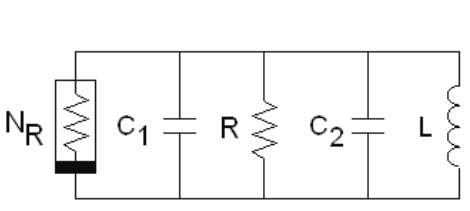
\includegraphics[width=0.9\textwidth]{Images/fig1(a).png}
		\caption{(a)}
		\label{fig:1a}
	\end{subfigure}%
	\begin{subfigure}[b]{0.5\textwidth}
		\centering
		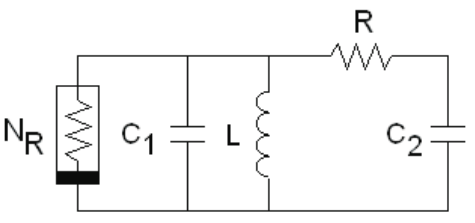
\includegraphics[width=0.9\textwidth]{Images/fig1(b).png}
		\caption{(b)}
		\label{fig:1b}
	\end{subfigure}
	% c and d
	\begin{subfigure}[b]{0.5\textwidth}
		\centering
		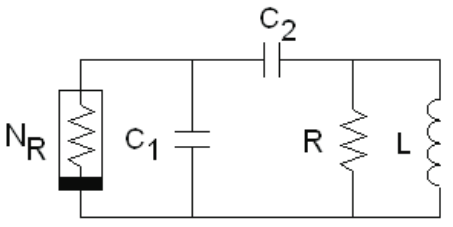
\includegraphics[width=0.9\textwidth]{Images/fig1(c).png}
		\caption{(c)}
		\label{fig:1c}
	\end{subfigure}%
	\begin{subfigure}[b]{0.5\textwidth}
		\centering
		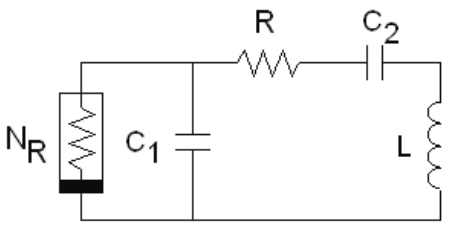
\includegraphics[width=0.9\textwidth]{Images/fig1(d).png}
		\caption{(d)}
		\label{fig:1d}
	\end{subfigure}
	% e and f
	\begin{subfigure}[b]{0.5\textwidth}
		\centering
		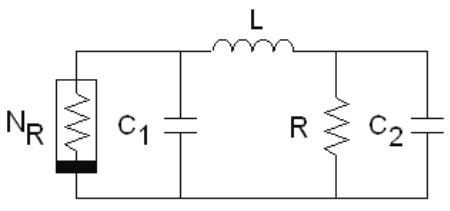
\includegraphics[width=0.9\textwidth]{Images/fig1(e).png}
		\caption{(e)}
		\label{fig:1e}
	\end{subfigure}%
	\begin{subfigure}[b]{0.5\textwidth}
		\centering
		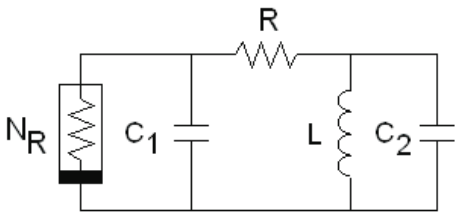
\includegraphics[width=0.9\textwidth]{Images/fig1(f).png}
		\caption{(f)}
		\label{fig:1f}
	\end{subfigure}
\end{figure}
\begin{figure}[H]
	\centering
	\caption{Fig 1. Possible configurations for circuit}
	% g and h
	\begin{subfigure}[b]{0.5\textwidth}
		\centering
		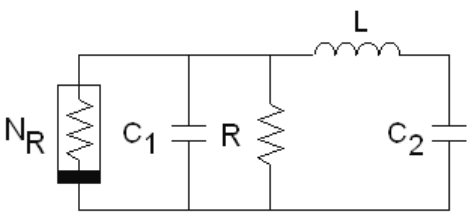
\includegraphics[width=0.9\textwidth]{Images/fig1(g).png}
		\caption{(g)}
		\label{fig:1g}
	\end{subfigure}%
	\begin{subfigure}[b]{0.5\textwidth}
		\centering
		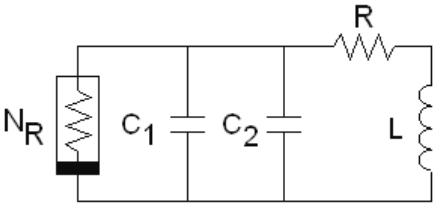
\includegraphics[width=0.9\textwidth]{Images/fig1(h).png}
		\caption{(h)}
		\label{fig:1h}
	\end{subfigure}
\end{figure}
Configuration (g) and (h) can be immediately rejected. \linebreak
In (g) the characteristic of resistance R can be absorbed in the characteristics of non-linear resistor $N_R$.
In (h) the $C_1$ and $C_2$ capacitances can be replaced by a single effective capacitor $C=C_1+C_2$. 
So in both of these configurations all circuit elements donot give unique contribution. Thus they can be rejected.\linebreak

For (a) and (b), the DC equilibrium calculations show that non-linear resistor gets short-circuited by the inductor. 
For (c) and (d), the DC equilibrium calculations show that non-linear resistor terminals are open.
So all the four configurations can be rejected. \linebreak

The remaining configuration (e) and (f) are both valid, but Chua selected configuration (f) because the RLC subcircuit generates oscillations.
%
%subsection 2.3
\subsection{Final Circuit}
The final Chua circuit is given as follows :
\begin{figure}[H]
	\centering
	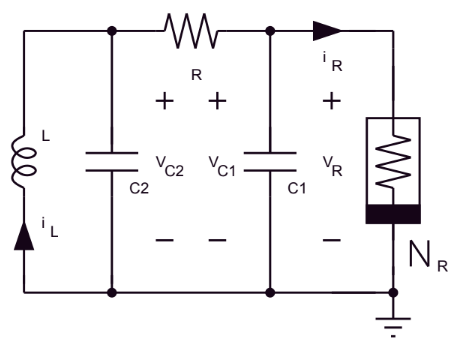
\includegraphics[width=0.6\textwidth]{Images/fig2_final.png}
	\caption{Fig 2. Chua's Circuit}
\end{figure}
%
%%%%%%%%%%%%%%%%%%%%%%%%%%%%%%%%%%%%%%%%%%%%%%%%%%%%%%%%%%%%
% SECTION 3 - STATE EQUATIONS AND SIMULATION
\section{State Equations and Simulations}
%subsection 3.1
\subsection{State Equations}
The equations of Chua's circuit are given as a system of three coupled differential equations :
\begin{align}
	C_1 \dfrac{dv_{C_1}}{dt}&=G\left( v_{C_2}-v_{C_1} \right)-g(v_{C_1}) \label{eq:1} \\
	C_2 \dfrac{dv_{C_2}}{dt}&=G\left( v_{C_1}-v_{C_2} \right)-i_L \label{eq:2}\\
	L \dfrac{i_L}{dt}&=-v_{C_2}\label{eq:3}
\end{align}
where, $G=\dfrac{1}{R}$ is the conductance, and $g(x)$ is a piece-wise linear function. It is given as :
\begin{align}
	g(v)&=m_0v+\dfrac{1}{2}(m_1-m_0)\left[ |v+B_p|-|v-B_p| \right] \label{eq:4}
\end{align}
where,
\begin{align*}
	m_0 &\implies \text{slope of outer region} \\
	m_1 &\implies \text{slope of inner region} \\
	B_P &\implies \text{breakpoints (both positive and negative values)}
\end{align*}
%
%subsection 3.2 - simulations
\subsection{Simulation}
The variables were redefined and all constants were taken to right hand side to make handling the equations easier.
\begin{align}
	\dfrac{dx}{dt}&=\dfrac{1}{C_1}\left\{ G\left( y-x \right)-g(x) \right\} \label{eq:5} \\
	\dfrac{dy}{dt}&=\dfrac{1}{C_2}\left\{ G\left( x-y \right)-z \right\} \label{eq:6} \\
	\dfrac{dz}{dt}&=-\dfrac{y}{L} \label{eq:7}
\end{align}
where,
\[ x \equiv v_{C_1} \quad y \equiv v_{C_2} \quad z \equiv i_L \]
The equation $g(x)$ remains the same as in (\myref{eq:4}).\linebreak
The equations are solved numerically using Runge Kutta 4 method in Python. All plots are made using Gnuplot.
%
%subsubsection 3.2.1 - Pyhton
\subsubsection{Python Codes}
The code for RK4 is as follows :
\lstinputlisting[language=Python]{/home/ashmita/Desktop/ASHMITA/APanda_Lib/chua_circuit_simulations.py}
The code inputs the three differential equations as a column vector F which is a function of x, y, z and t (time). x, y and z are arranged as column vector b. For the first iterations, it has the initial values. 
h is the increment factor. N is the number of iterations. $t_0$ is the initial time value. \linebreak

The `append.file()' function saves the data points (t, x, y and z) after each iteration in a file (filename provided to function as variable `name'). All codes for manipulation with files is as follows :
\lstinputlisting[language=Python]{/home/ashmita/Desktop/ASHMITA/APanda_Lib/handling_files.py}
%
% subsubsection 3.2.2 - plots with dimensionless constants
\subsubsection{Plots with Dimensionless Constants}
The following values were used for the constants :
\[ G=0.7 \quad C_1=1/9 \quad C_2=1 \quad L=1/7 \quad B_p=1 \quad m_0=-0.5 \quad m_1=-0.8 \]
The function g(v) in (\myref{eq:4}) can be plotted using the constants. 
\begin{figure}[H] %fig 3
	\centering
	\includegraphics[width=0.75\textwidth,height=0.3\textheight]{Plots/fig3_g(v).png}
	\caption{Fig 3. Three Segment Linear Function : g(v)}
\end{figure}
The code for defining the function, initial values and calling the function is :
\lstinputlisting[language=Python]{/home/ashmita/Desktop/ASHMITA/NISER Study/7th Semester/Open Lab/Non-Linear Circuit/Dimensionless/dimensionless_chua.py}
The data file obtained is plotted using Gnuplot.
\begin{figure}[H] % fig 4
	\centering
	\includegraphics[width=0.8\textwidth]{Plots/fig4_dimensionless_plot.png}
	\caption{Fig 4. 3D plot of $v_{C_1}$ vs $v_{C_2}$ for dimensionless constants}
\end{figure}
Thus, we do obtain a double scroll attractor for the Chua Circuit. In principle, the Chua Ciruit does exhibit chaotic behaviour. 
%
%subsubsection 3.2.3 - Varying R with dimensionful constants
\subsubsection{Varying R with Dimensionful Constants}
Now, we will attempt to use constants which represent actual dimensionful values and try to observe how the graph changes when we change the value of resistance $R$. \linebreak

We will define conversion factors to relate the value of our constants to values of actual electronic circuit components. Current will be measured in Amperes(A), potential differences in Volts(V), capacitances in Farads(F), inductance in Henry(H) and resistance in Ohm($\Omega$). Resistivity is expressed in Siemens(S)\linebreak
If we want currents of milliamperes to be in the circuit, we will adjust all current values by 1000. It will thus increase resistances and inductance by 1000, while decreasing capacitances by the same factor. Also, we can also rescale the values of time by some factor k in (\myref{eq:3}). This will leave all resistances unaffected, and all capacitors and inductors will be scaled by same factor k. For ease of using values in the code, k is chosen to be $10^{-4}$, i.e., all capacitances and inductances are rescaled by $10^{-4}$. This gives us the final conversion factors as :
\begin{align*}
	R & : 1 \equiv 1000 \Omega = 1k\Omega \\
	C_1, C_2 & : 1 \equiv 10^{-7} F = 100 nF \\
	L & : 1 \equiv 10^{-1} H = 100 mH \\
	m_0, m_1 & : 1 \equiv 10^{-3} S = 1 mS \\
	B_p & : 1 \equiv 1 V
\end{align*}
So, the constants used in the previous part correspond to :
\begin{equation*}
	R=1.43k\Omega \; ;  C_1=11.11 nF \; ; C_2=100 nF \; ; L=14.29 mH \; ; B_p = 1V \; ; m_0 = -0.5 mS \; ; m_1 = -0.8 mS
\end{equation*}
We will now attempt to vary R and observe how the output changes. \linebreak
The code for defining the function, initial values, varying R values and calling the function is :
\lstinputlisting[language=Python]{/home/ashmita/Desktop/ASHMITA/NISER Study/7th Semester/Open Lab/Non-Linear Circuit/Varying R/varying_R.py}
Plotting the data files obtained in Gnuplot. 
\begin{figure}[H] %fig 5
	\centering
	% a and b
	\caption{Fig 5. R Bifurcation in Theoretical Chua Circuit using a Three Segment Non-Linear Resistance}
	\begin{subfigure}[b]{0.5\textwidth}
		\centering
		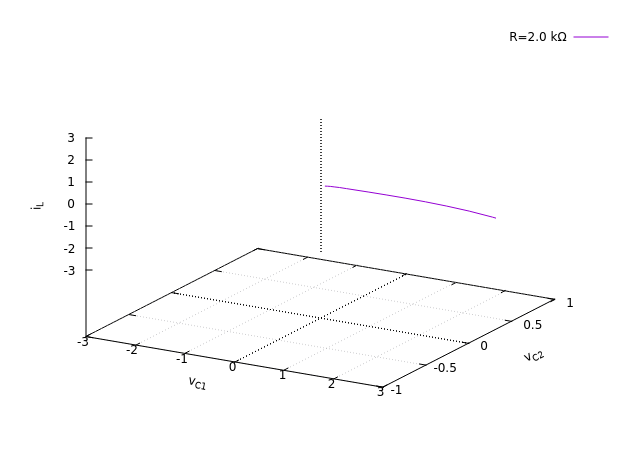
\includegraphics[width=\textwidth]{Plots/fig5(a)_2k.png}
		\caption{(a) $R=2.0k\Omega$}
	\end{subfigure}%
	\begin{subfigure}[b]{0.5\textwidth}
		\centering
		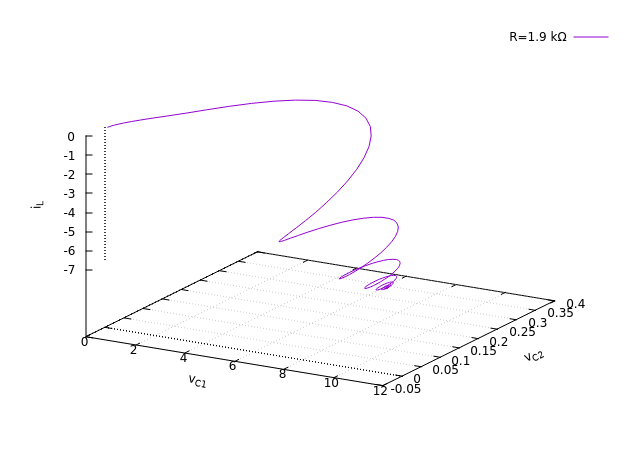
\includegraphics[width=\textwidth]{Plots/fig5(b)_1.9k.png}
		\caption{(b) $R=1.9k\Omega$}
	\end{subfigure}
\end{figure}
\begin{figure}[H] %fig 5 contd
	\centering
	% c and d
	\begin{subfigure}[b]{0.5\textwidth}
		\centering
		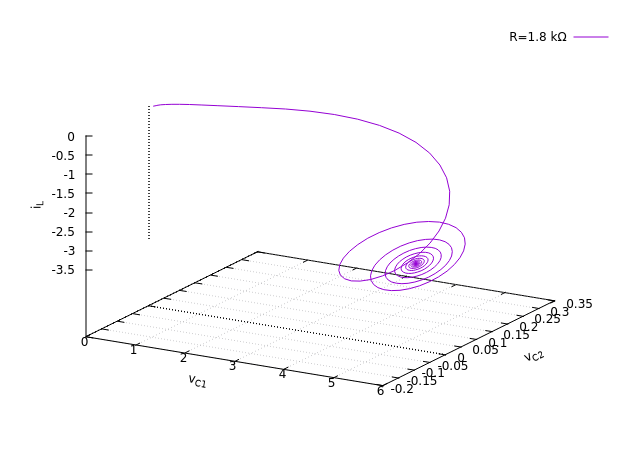
\includegraphics[width=\textwidth]{Plots/fig5(c)_1.8k.png}
		\caption{(c) $R=1.8k\Omega$}
	\end{subfigure}%
	\begin{subfigure}[b]{0.5\textwidth}
		\centering
		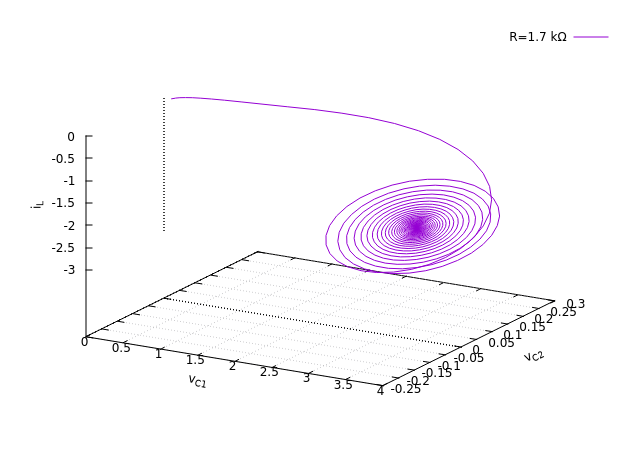
\includegraphics[width=\textwidth]{Plots/fig5(d)_1.7k.png}
		\caption{(d) $R=1.7k\Omega$}
	\end{subfigure}
	% e and f
	\begin{subfigure}[b]{0.5\textwidth}
		\centering
		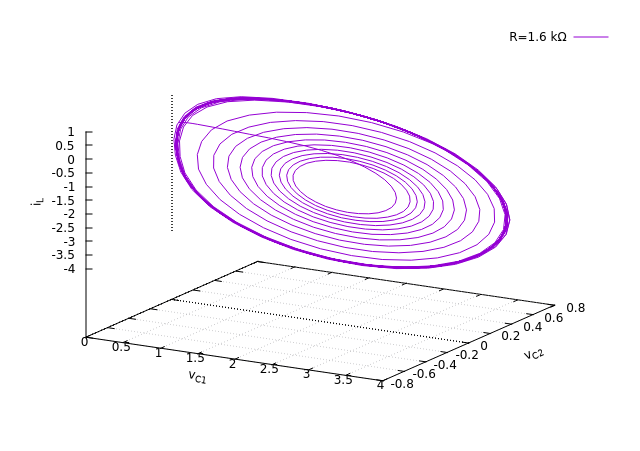
\includegraphics[width=\textwidth]{Plots/fig5(e)_1.6k.png}
		\caption{(e) $R=1.6k\Omega$}
	\end{subfigure}%
	\begin{subfigure}[b]{0.5\textwidth}
		\centering
		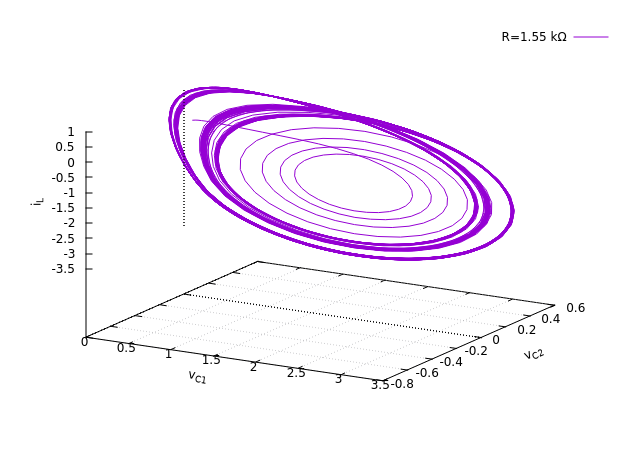
\includegraphics[width=\textwidth]{Plots/fig5(f)_1.55k.png}
		\caption{(f) $R=1.55k\Omega$}
	\end{subfigure}
	% g and h
	\begin{subfigure}[b]{0.5\textwidth}
		\centering
		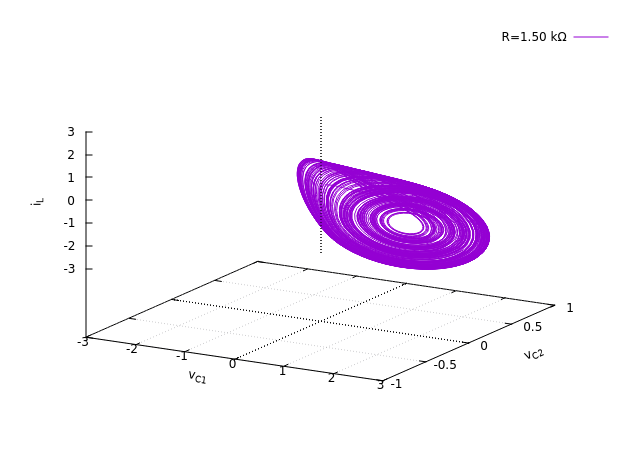
\includegraphics[width=\textwidth]{Plots/fig5(g)_1.5k.png}
		\caption{(g) $R=1.5k\Omega$}
	\end{subfigure}%
	\begin{subfigure}[b]{0.5\textwidth}
		\centering
		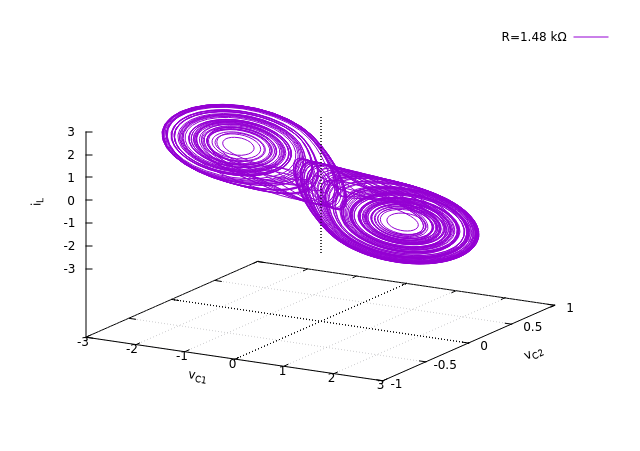
\includegraphics[width=\textwidth]{Plots/fig5(i)_1.48k.png}
		\caption{(h) $R=1.48k\Omega$}
	\end{subfigure}
	% i and j
	\begin{subfigure}[b]{0.5\textwidth}
		\centering
		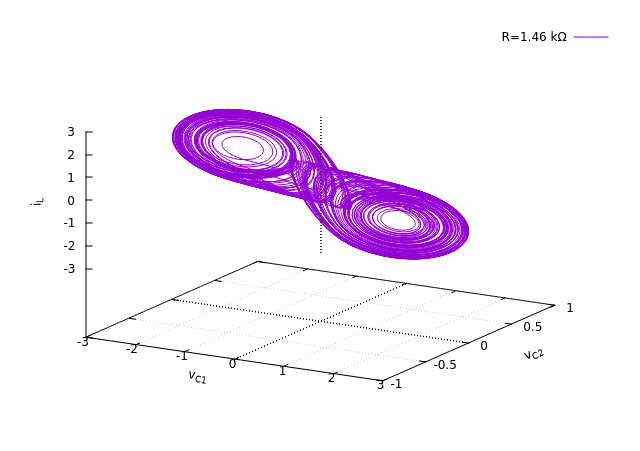
\includegraphics[width=\textwidth]{Plots/fig5(k)_1.46k.png}
		\caption{(i) $R=1.46k\Omega$}
	\end{subfigure}%
	\begin{subfigure}[b]{0.5\textwidth}
		\centering
		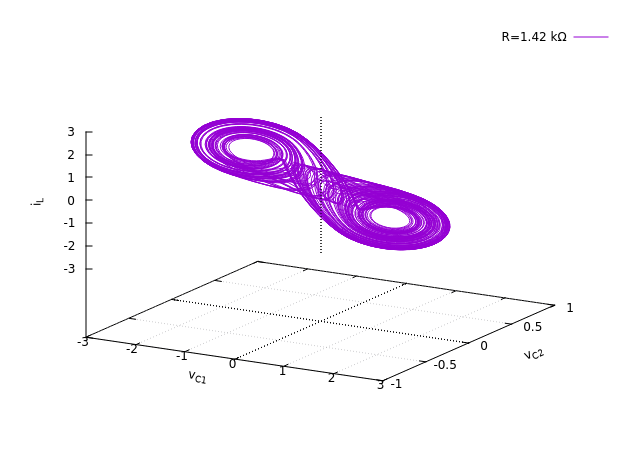
\includegraphics[width=\textwidth]{Plots/fig5(n)_1.42k.png}
		\caption{(j) $R=1.42k\Omega$}
	\end{subfigure}
\end{figure}
%
\begin{figure}[H] %fig 5 contd
	\centering
	% k and l
	\begin{subfigure}[b]{0.5\textwidth}
		\centering
		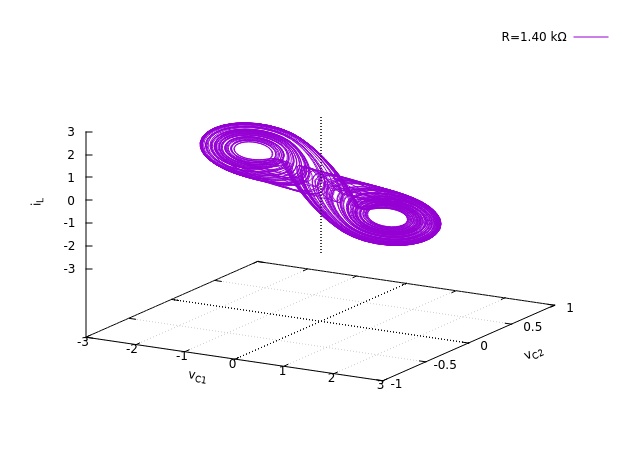
\includegraphics[width=\textwidth]{Plots/fig5(o)_1.40k.png}
		\caption{(k) $R=1.4k\Omega$}
	\end{subfigure}%
	\begin{subfigure}[b]{0.5\textwidth}
		\centering
		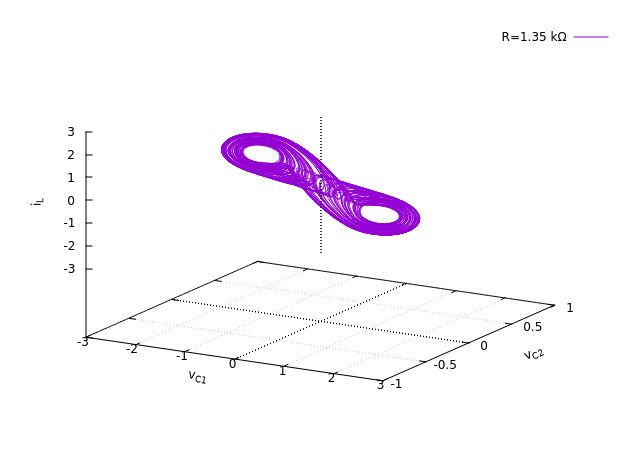
\includegraphics[width=\textwidth]{Plots/fig5(p)_1.35k.png}
		\caption{(l) $R=1.35k\Omega$}
	\end{subfigure}
	% m and n
	\begin{subfigure}[b]{0.5\textwidth}
		\centering
		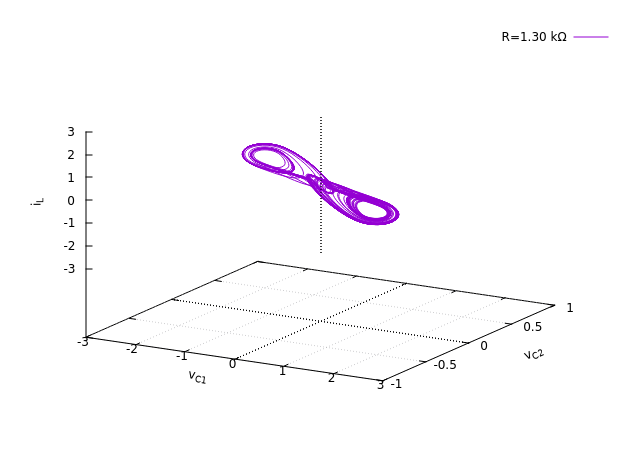
\includegraphics[width=\textwidth]{Plots/fig5(q)_1.30k.png}
		\caption{(m) $R=1.3k\Omega$}
	\end{subfigure}%
	\begin{subfigure}[b]{0.5\textwidth}
		\centering
		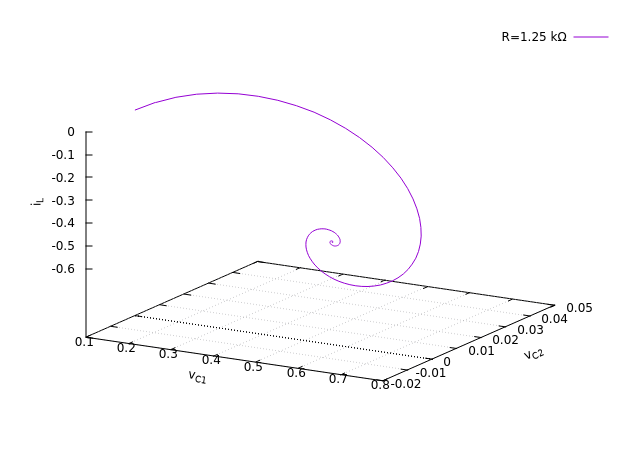
\includegraphics[width=\textwidth]{Plots/fig5(r)_1.25k.png}
		\caption{(n) $R=1.25k\Omega$}
	\end{subfigure}
	% o and p
	\begin{subfigure}[b]{0.5\textwidth}
		\centering
		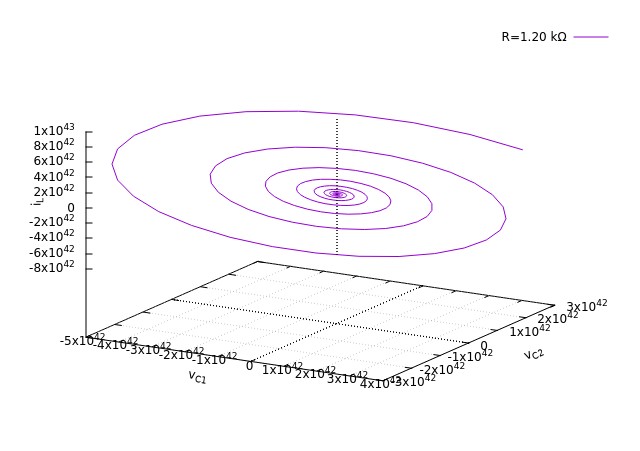
\includegraphics[width=\textwidth]{Plots/fig5(s)_1.20k.png}
		\caption{(o) $R=1.2k\Omega$}
	\end{subfigure}%
	\begin{subfigure}[b]{0.5\textwidth}
		\centering
		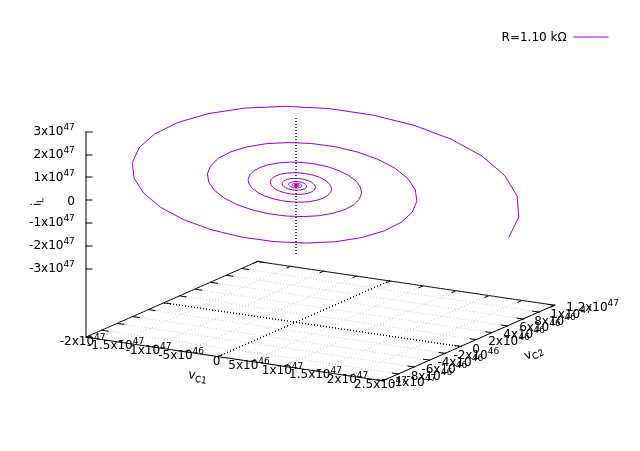
\includegraphics[width=\textwidth]{Plots/fig5(t)_1.10k.png}
		\caption{(p) $R=1.1k\Omega$}
	\end{subfigure}
\end{figure}
We observe that $R=2.0 k\Omega$ shows DC Equilibrium. As resistance is reduced, the characteristics looks like an unbounded spiral. \linebreak
The Rossler Attractor forms around $R=1.5 k\Omega$ and the Double Scroll Attractor is first formed at $R=1.48k\Omega$. As the resistance is further reduced, the size of the double scroll also decreases. \linebreak
By $R=1.25k\Omega$ the double scroll character is lost, and for lower resistances the graphs show a spiral with no upper bound. The values of $v_{C_1}$, $v_{C_2}$ and $i_L$ apparently take values in the ranges of $10^{43}$ and $10^{47}$. This is not physically possible.
%
%subsection 4 - Problems with Simulation
\subsection{Problems with Simulation}
The current simulation of the Chua Circuit is not physically viable, as is evident from the graphs obtained for various values of resistance. It predicts that except for a small window of resistance values (from $R=1.5k\Omega$ to $R=1.3k\Omega$) the values of voltages and current is not bounded. \linebreak

The problems arises because we have failed to take into account the fact that all physical resistors are eventually passive, i.e., for large enough values of voltages applied across its terminals, the power consumed by the resistor becomes positive. \linebreak
In our current equation (\myref{eq:4}) and graph of g(v), we see that the condition of eventual passivisity has not been taken into account. The power consumed by the resistor is negative for all values of voltages.
%%%%%%%%%%%%%%%%%%%%%%%%%%%%%%%%%%%%%%%%%%%%%%%%%%%%%%%%%%
%section 4 - Simulation to Practical Design
\section{Simulation to Practical Design}
%%
%subsection 4.1 - Negative Resistance
\subsection{Negative Resistance}
To implement a Chua Circuit practically we first need to construct negative resistances which when put together, follows the characteristics of $g(v)$ graph. One way to construct a negative resistance is to connect three positive linear resistors to a voltage controlled voltage source (VCVS).
%
%subsubsection 4.1.1-VCVS
\subsubsection{Voltage Controlled Voltage Source}
A VCVS is defined to be an ideal circuit element with two input and two output terminals such that no current flows between the input terminals and voltage across output terminals is dependent on the volatge across input terminals.
\[ v_o= f(v_d) \]
$f(.)$ could have any functional dependence, but the simplest non-trivial relation occurs when it is linear. 
\begin{figure}[H]
	\centering
	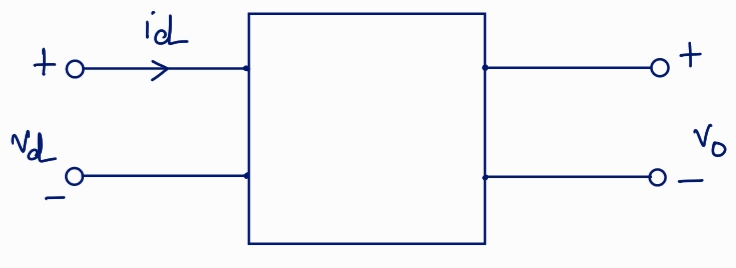
\includegraphics[width=0.7\textwidth]{Images/fig6_vcvs.png}
	\caption{Fig 6. Voltage Controlled Voltage Source}
\end{figure} 
%
%subsubsection 4.1.2 - negative resistance using VCVS
\subsubsection{Negative Resistance using ideal VCVS}
The circuit diagram to build a negative resistance using an ideal VCVS and three linear resistors is given as follows :
\begin{figure}[H]
	\centering
	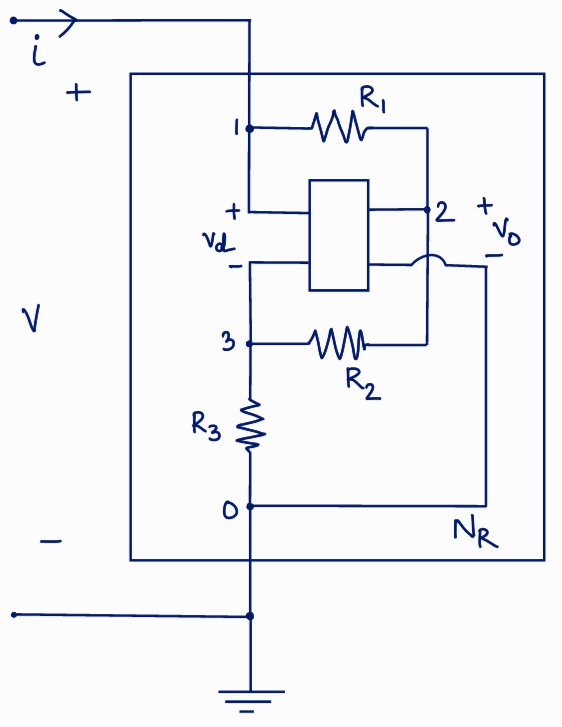
\includegraphics[width=0.5\textwidth]{Images/fig7_Nr with vcvs.png}
	\caption{Fig 7. Negative Resistance using VCVS}
\end{figure}
Let us assume the VCVS follows a linear relationship :
\begin{equation}
	v_o=Av_d \label{eq:8}
\end{equation}
A is some proportionality constant. \linebreak

Now, Kirchoff's Current Law (KCL) says that \textit{for any node in an electrical circuit, the sum of the currents entering the node is equal to the sum of the currents leaving the node}. \linebreak

Applying KCl on node (1) (in Fig 7):
\begin{equation}
	i=i_1 \quad ; \quad  i_1=\dfrac{v-v_o}{R_1} \label{eq:9}
\end{equation}
We can write this because no current goes inside VCVS.\linebreak

Now, Kirchoff's Voltage Law (KVL) says that \textit{if we move around a closed loop in a fixed direction then the sum of all the potential differences around the loop is zero.} \linebreak

Applying KVL along loop 1-2-3-0 (in Fig 7):
\begin{align}
	v&=v_d + i_3R_3 \label{eq:10} \\
	i_3&=\dfrac{v_o}{R_2+R_3} \label{eq:11}
\end{align}
Using (\myref{eq:11}) in (\myref{eq:10}) :
\begin{align}
	v&=v_d + \dfrac{A R_3 v_d}{R_2+R_3} = \dfrac{R_2+(1+A)R_3}{R_2+R_3}v_d \nonumber \\
	\intertext{Now, using (\myref{eq:8}) in the above equation : }
	\therefore v&= \left\{ \dfrac{R_2+(1+A)R_3}{A(R_2+R_3)} \right\}v_o \label{eq:12}
\end{align}
We can now calculate the current $i$ using (\myref{eq:9}) :
\begin{align*}
	i&=\dfrac{v}{R_1}-\dfrac{v_o}{R_1} \\
	\intertext{Using equation of $v$ and $v_o$ (\myref{eq:12}) :}
	\implies i &= \dfrac{v}{R_1}-\dfrac{1}{R_1}\left\{ \dfrac{A(R_2+R_3)}{R_2+(1+A)R_3}v \right\} \\
	\implies i &= \dfrac{vR_2+vR_3+vAR_3-AR_2v-AR_3v}{R_1\left[ R_2+(1+A)R_3 \right]}
\end{align*}
So we finally obtain :
\begin{equation}
	\therefore i = \left\{ \dfrac{R_2(1-A)+R_3}{R_1\left[ R_2+(1+A)R_3 \right] } \right\} \label{eq:13}
\end{equation}
Now if we take A to be very large, $A\gg 1$, greater than $R_1, R_2$ and $R_3$, we can write :
\begin{align*}
	\implies i & \thickapprox \dfrac{-R_2A+R_3}{R_1(R_2+R_3A)}v \\
	\intertext{Also, as $R_2A \gg R_3$ and $R_1R_3A \gg R_1R_2$ :}
	\implies i & \thickapprox -\dfrac{R_2A}{R_1R_3A}v \thickapprox -\dfrac{R_2}{R_1R_3}v
\end{align*}
We can now set $R_1=R_2$, and we obtain :
\begin{equation}
	i=-\dfrac{1}{R_3}v \label{eq:14}
\end{equation}
Thus it appears that the segment $N_R$ (in Fig 7) now has negative resistance $-R_3$. 
%
%subsubsecrion 4.1.3 - opamps as VCVS
\subsubsection{Op-Amps as VCVS}
An op-amp is the practical or real-life approximation of a VCVS. The voltage applied across inverting and non-inverting terminals produces voltage at output terminal, if we take the reference terminal to be ground.
\begin{figure}[H]
	\centering
	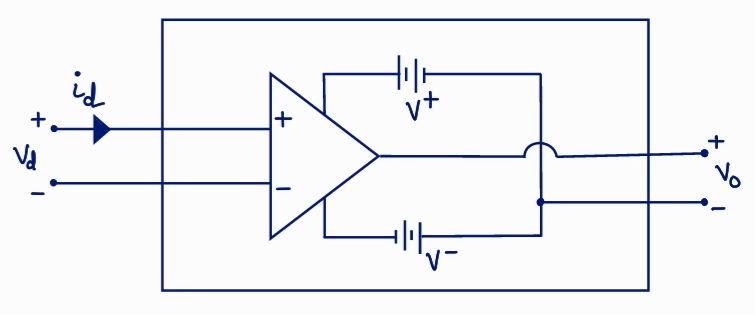
\includegraphics[width=0.6\textwidth]{Images/fig8_opamp as vcvs.png}
	\caption{Fig 8. Op-amp as VCVS}
\end{figure}
Ideal opamps there is no current entering the circuit, i.e., $i_d=0$ and the loop gain is infinite. But typically, most opamps produce output voltages 100,000 times larger than the potential difference between input terminals. \linebreak

The output of a opamp becomes constant at some values of $v_d=\pm E_{sat}$.
\begin{align*}
	\text{For } v_d\geq \dfrac{E_{sat}}{A}+v_{OS} & \quad \text{: positive saturation region} \\
	\text{For } v_d\leq-\dfrac{E_{sat}}{A}+v_{OS} & \quad \text{: negative saturation region} \\
	\text{For } -\dfrac{E_{sat}}{A}+v_{OS}< v_d < \dfrac{E_{sat}}{A}+v_{OS} & \quad \text{: linear region}
\end{align*}
$v_{OS}$ is the offset voltage. 
\begin{figure}[H]
	\centering
	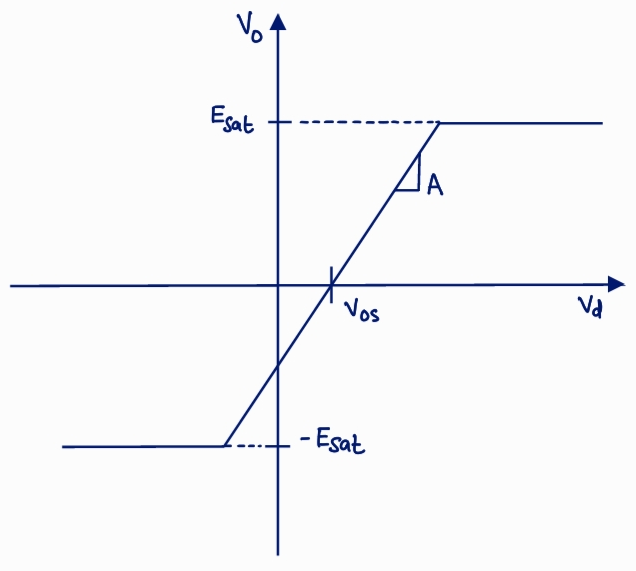
\includegraphics[width=0.5\textwidth]{Images/fig9_opamp characteristics.png}
	\caption{Fig 9. Output Characteristics of an Op-Amp}
\end{figure}
From here on, we will assume :
\[ v_{OS} =0 \quad ; \quad i_d=0 \quad ; \quad v_o=f(v_d) \]
%
%subsubsection 4.1.4
\subsubsection{Negative Resistance using Op-Amps}
We can build a negative resistance using the analysis we did previously, while using Op-Amp as VCVS.
\begin{figure}[H]
	\centering
	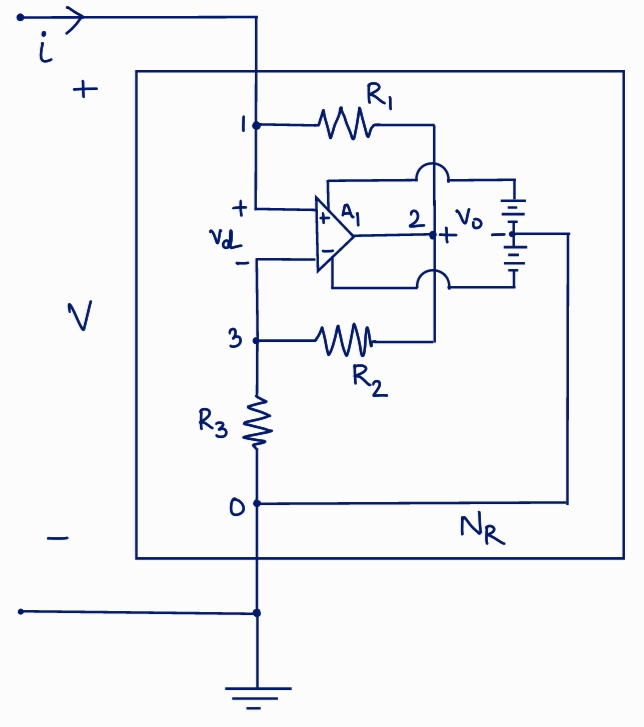
\includegraphics[width=0.5\textwidth]{Images/fig10_negative resistance using opamp.png}
	\caption{Fig 10. Negative Resistance using Op-Amps}
\end{figure}
From previous circuit analysis we have :
\begin{equation}
	i=\dfrac{v-v_o}{R_1} \quad ; \quad v=v_d+\dfrac{R_3}{R_2+R_3}v_o \quad ; \quad v_o = Av_d \label{eq:15}
\end{equation}
As now we have an op-amp, there are three distinct regions depending on the voltage behavior :
\begin{align*}
	\text{Negative Saturation} & : \qquad  v_o = -E_{sat} \qquad ; \qquad v_d \leq -\dfrac{E_{sat}}{A} \\
	\text{Linear Region} & : \qquad  v_o=Av_d \qquad ; \qquad -\dfrac{E_{sat}}{A} < v_d < \dfrac{E_{sat}}{A} \\
	\text{Positive Saturation} & : \qquad v_0=E_{sat} \qquad ; \qquad v_d\geq \dfrac{E_{sat}}{A} \\
\end{align*}
\textbf{\uline{Positive Saturation}} \linebreak %positive saturration
In the positive saturation region the output voltage is fixed at $E_{sat}$, even if the input changes.
\begin{equation}
	v_o = E_{sat} \qquad ; \qquad v_d \geq \dfrac{E_{sat}}{A} \label{eq:16}
\end{equation}
From (\myref{eq:15}) and (\myref{eq:16}), we have equation of current as :
\begin{equation}
	i=\dfrac{v}{R_1}-\dfrac{E_{sat}}{R_1} \label{eq:17}
\end{equation}
We can write the equation for voltage as :
\begin{align*}
	v&= v_d+\dfrac{R_3}{R_2+R_3}v_o \\
	\implies v & \geq \dfrac{E_{sat}}{A}+\dfrac{R_3}{R_2+R_3}E_{sat} \\
	\implies v & \geq E_{sat}\left\{ \dfrac{R_2+R_3+AR_3}{A(R_2+R_3)} \right\}
\end{align*}
So we finally obtain :
\begin{equation}
	v \geq \left\{ \dfrac{R_2+(1+A)R_3}{A(R_2+R_3)} \right\} E_{sat} \label{eq:18}
\end{equation}
So the minimum value of valid $v$ for positive saturation, or the positive breakpoint is given as :
\begin{equation}
	B^+_P = \dfrac{R_2+(1+A)R_3}{A(R_2+R_3)} E_{sat} \label{eq:19}
\end{equation}
Now if A is very large, we have $(1+A)R_3+R_2 \longrightarrow AR_3$. So we obtain the breakpoint as :
\begin{equation}
	B^+_P \simeq \dfrac{R_3}{R_2+R_3}E_{sat} \label{eq:20}
\end{equation}
Slope of the graph is given as :
\begin{equation}
	m_o=\dfrac{1}{R_1} \label{eq:21}
\end{equation}
\textbf{\uline{Negative Saturation}} \linebreak %negative saturation
In negative saturation, $v_o=-E_{sat}$. As all other equations remain same, we have the breakpoint as :
\begin{equation}
	B^-_P = - \dfrac{R_2+(1+A)R_3}{A(R_2+R_3)}E_{sat} \label{eq:22}
\end{equation}
For very large A, we get the breakpoint as :
\begin{equation}
	B^-_P \simeq -\dfrac{R_3}{R_2+R_3}E_{sat} \label{eq:23}
\end{equation}
The slope is still $m_o$. \linebreak
\textbf{\uline{Linear Region}} \linebreak %linear region
In the linear region, we have the standard circuit analysis we did before given in (\myref{eq:15}). \linebreak
Writing voltage $v_d$ in terms of $v$ :
\begin{align*}
	v&=v_d+\dfrac{R_3}{R_2+R_3}v_o \\
	\implies v &= v_d+\dfrac{R_3}{R_2+R_3}Av_d \\
	\implies v&= \dfrac{R_2+(1+A)}{R_2+R_3} v_d 
\end{align*}
Therefore, we obtain :
\begin{equation}
	v_d= \dfrac{R_2+R_3}{R_2+(1+A)R_3}v \label{eq:24}
\end{equation}
Using this (\myref{eq:24}) to find current $i$ :
\begin{equation}
	i = \dfrac{(1-A)R_2+R_3}{R_1\left[ R_2+(1+A)R_3 \right]}v \label{eq:25}
\end{equation}
For large A, we have :
\begin{equation}
	i \simeq - \dfrac{R_2}{R_1R_3}v \label{eq:26}
\end{equation}
The linear region is characterised by :
\begin{align*}
	& -\dfrac{E_{sat}}{A}<v_d<\dfrac{E_{sat}}{A} \\
	\implies & -\dfrac{E_{sat}}{A}<\dfrac{R_2+R_3}{R_2+(1+A)R_3}v < \dfrac{E_{sat}}{A} \\
	\intertext{For $v$ : }
	\therefore & -E_{sat}\dfrac{R_2+(1+A)R_3}{A(R_2+R_3)} < v < E_{sat} \dfrac{R_2+(1+A)R_3}{A(R_2+R_3)} \\
	\intertext{For large A, we have :}
	\implies & -E_{sat}\dfrac{R_3}{R_2+R_3}<v<E_{sat}\dfrac{R_3}{R_2+R_3} \\
	\intertext{From (\myref{eq:20}) and (\myref{eq:23}) :}
	\therefore & B^-_P < v < B^+_P 
\end{align*}
Thus, when voltage $v$ lies between breakpoints, the op-amp functions in the linear region. \linebreak
Slope of the I-V graph in this region is :
\begin{equation}
	m_1=-\dfrac{R_2}{R_1R_3} \label{eq:27}
\end{equation}
The I-V characteristics of negative resistance implemented using op-amps should be of the form :
\begin{figure}[H]
	\centering
	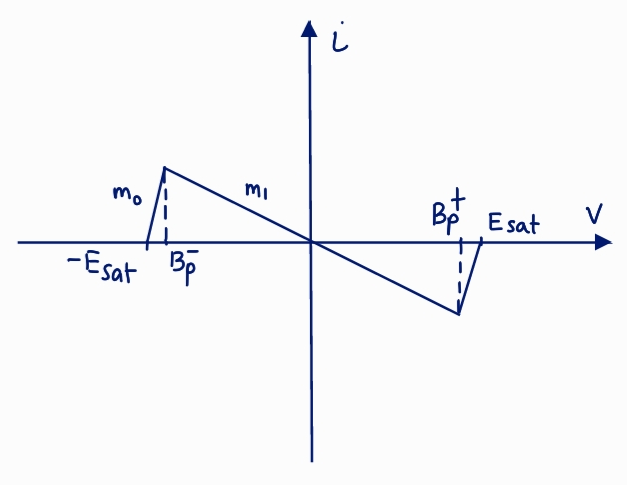
\includegraphics[width=0.5\textwidth]{Images/fig11_negative characteristics.png}
	\caption{Fig 11. Expected I-V Characteristics of Negative Resistance}
\end{figure}
%%
%subsection 4.2 - Non-Linear Resistance
\subsection{Non-Linear Resistance}
Now that we have the negative resistances, we would like to implement our Non-Linear resistance to be used in the circuit. To do so, we need to put two negative resistances in parallel. \linebreak
$N_{R_1}$ includes resistances $R_1$, $R_2$ and $R_3$. It has slopes $m_{01}$, $m_{11}$ and breakpoints $\pm B_{P1}$. \linebreak
$N_{R_2}$ includes resistances $R_4$, $R_5$ and $R_6$. It has slopes $m_{02}$, $m_{12}$ and breakpoints $\pm B_{P2}$. \linebreak

We will assume $R_1=R_2$ and $R_4=R_5$. 
\begin{figure}[H]
	\centering
	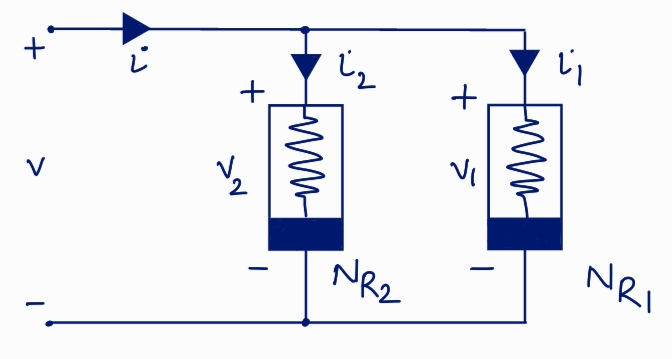
\includegraphics[width=0.6\textwidth]{Images/fig12_nonlinear.png}
	\caption{Fig 12. Non-linear Resistance}
\end{figure}
So for $N_{R_1}$ we have :
\begin{equation}
	m_{01}=\dfrac{1}{R_1} \qquad ; \qquad m_{11}=-\dfrac{1}{R_3} \qquad ; \qquad B_{P1}=\pm \dfrac{R_3}{R_2+R_3}E_{sat} \label{eq:28}
\end{equation}
For $N_{R_2}$ we have :
\begin{equation}
	m_{02}=\dfrac{1}{R_4} \qquad ; \qquad m_{12}= -\dfrac{1}{R_6} \qquad ; \qquad B_{P2}= \pm \dfrac{R_6}{R_5+R_6}E_{sat} \label{eq:29} 
\end{equation}
Slopes of $N_{R_1}$ and $N_{R_2}$ are connected to the slopes of the combined graph is :
\begin{equation}
	m_{11}+m_{02}=m_0 \qquad ; \qquad m_{11}+m_{12}=m_1 \label{eq:30}
\end{equation}
The expected I-V graph of non-linear resistance is as follows :
\begin{figure}[H]
	\centering
	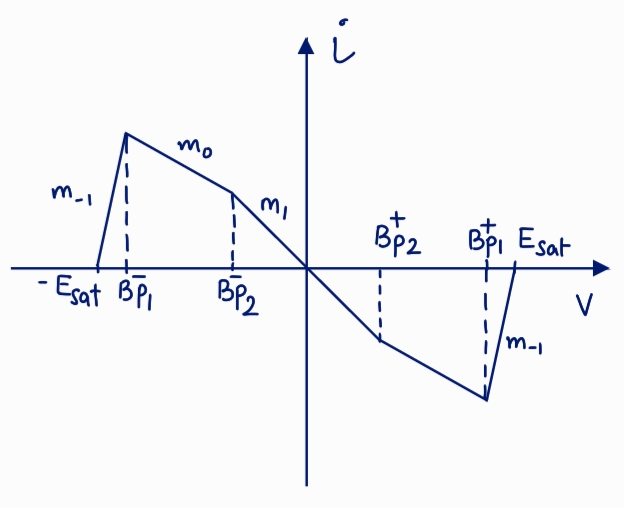
\includegraphics[width=0.6\textwidth]{Images/fig13_nonlinear characteristics.png}
	\caption{Fig 13. Expected I-V Characteristics of non-linear resistance}
\end{figure}
%%%%%%%%%%%%%%%%%%%%%%%%%%%%%%%%%%%%%%%%%%%%%%%%%%%%%%
%section 5 - Practical Implementation using LTSpice
\section{Practical Implementation with LTSpice}
LTSpice was used to practically implement the Chua Ciruit. The circuit design is used from the paper by Kennedy[1] (Fig 101. \linebreak

All op-amps used are TL082, which are downloaded as a third-party tool from the website \url{http://www.chaotic-circuits.com/simulating-electronic-circuits/}[3] and implemented into the circuit.\linebreak
%%
%subsection 5.1 - Component Values
\subsection{Setting Component Values}
9V voltage sources were used to power the op-amps. The values of resistances, capacitors and inductors used to implement the circuit is as follows :
\begin{align*}
	\intertext{\textbf{For $\bm{N_{R_1}}$ :}}
	R_1 &= 220\Omega \pm 5\% \\
	R_2 &= 220\Omega \pm 5\% \\
	R_3 &= 2.2k\Omega \pm 5\% \\
	\intertext{\textbf{For $\bm{N_{R_2}}$ :}}
	R_4 &= 22k\Omega \pm 5\% \\
	R_5 &= 22k\Omega \pm 5\% \\
	R_6 &= 3.3k\Omega \pm 5\% \\ 
	\intertext{\textbf{Rest of the circuit elements :}}
	C_1 &= 10nF \pm 5\% \\
	C_2 &= 100nF \pm 5\% \\
	L &= 18mH \pm 10\% \\
	R &= 2.2k\Omega \text{ to } 1.48k\Omega 
\end{align*}
$R$ is varied from $2.2k\Omega$ to $1.48k\Omega$ to observe the various stages of the bifurcation sequence. 
%%
%subsection 5.2 - Negative Resistance
\subsection{Negative Resistances}
First the negative resistances are individually implemented in LTSpice to ensure they function as we theoretically expect them to. The saturation voltage ($E_{sat}$) for TL082 and breakpoints for both resistors is also obtained. \linebreak

To measure the current through the non-linear resistor, a small resistance of value $R=100\Omega$ is put in series. The I-V graph of non-linear resistor is obtained on plotting input voltage and current measured across $R$. 
%
%subsubsection 5.2.1 - N_{R_1}
\subsubsection{N\textsubscript{R1}}
$N_{R_1}$ was implemented using LTSpice. $V_3$ is a variable DC voltage source and $R$ is a small current-sensing resistance.
\begin{figure}[H]
	\centering
	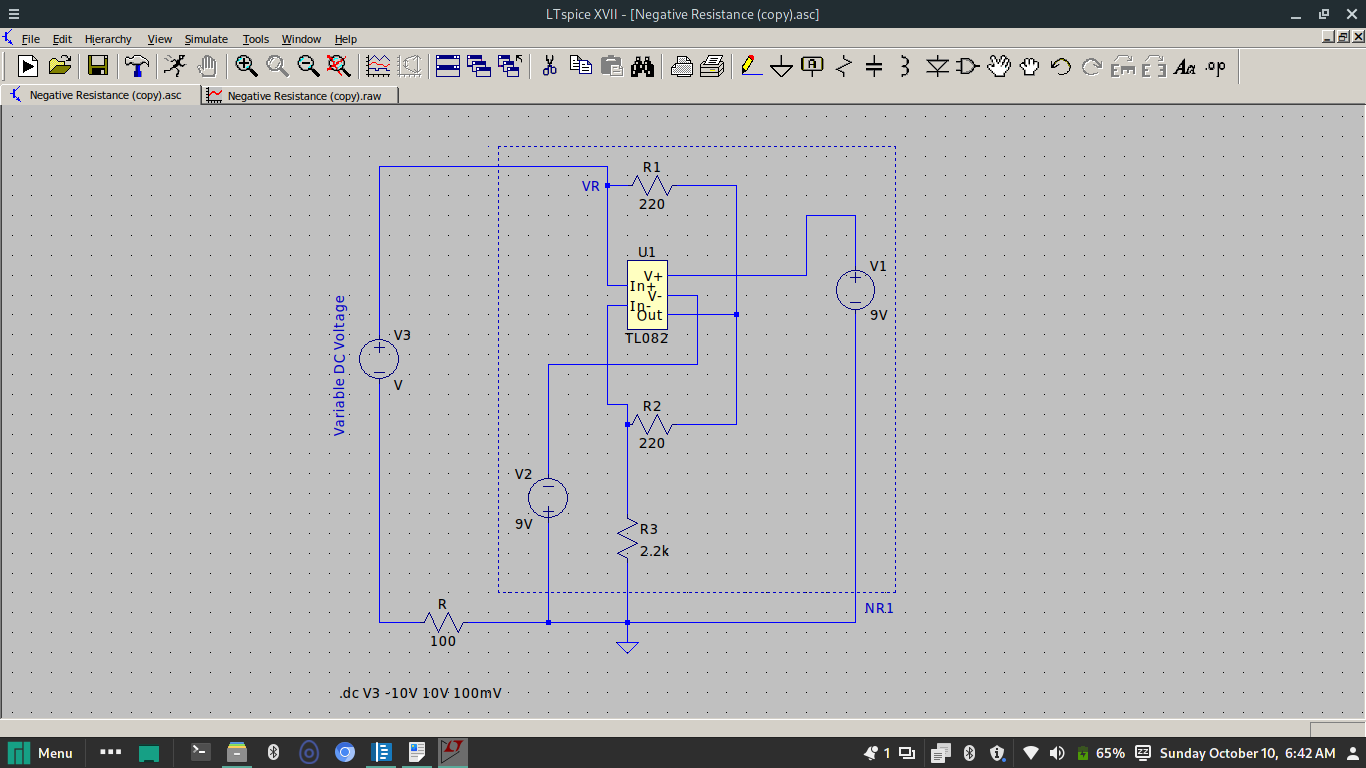
\includegraphics[width=\textwidth]{LTSpice/NR1_circuit.png}
	\caption{Fig 14. $N_{R_1}$ circuit}
\end{figure}
The corresponding I-V Graph is obtained on running the circuit in DC Sweep mode from -10V to 10V with intervals of 100mV. The saturation volatge $E_{sat}$ is observed to be $\pm 7.48V$.
\begin{figure}[H]
	\centering
	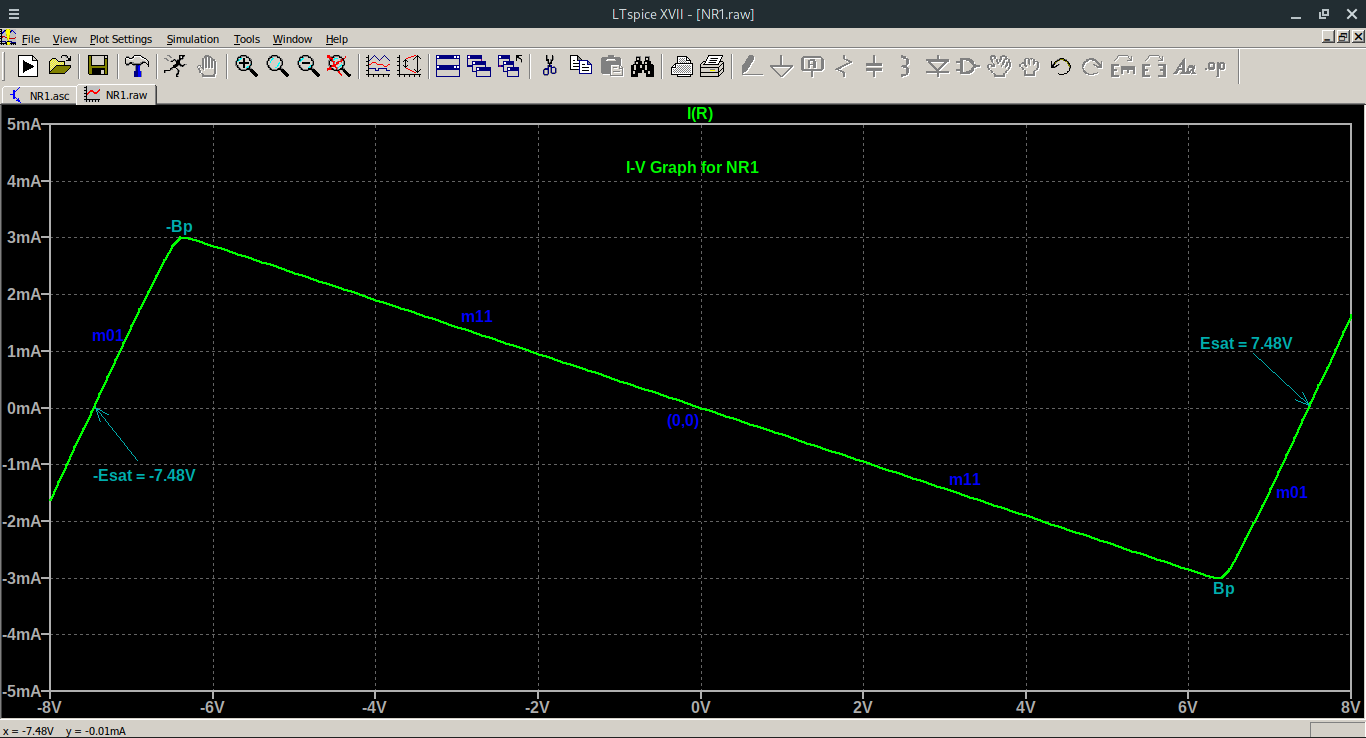
\includegraphics[width=\textwidth]{LTSpice/NR1_plot.png}
	\caption{Fig 15. I-V Characteristics of $N_{R_1}$}
\end{figure}

The values of slopes and breakpoints for $N_{R_1}$ are obtained from (\myref{eq:28}) as :
\begin{align*}
	E_{sat}&=\pm 7.48V \\
	m_{01}&=4.545\times 10^{-3} S = 4.545 mS \\ 
	m_{11}&= -4.545\times 10^{-4} S = -0.4545 mS \\
	B_{P1}&= \pm 6.8V 
\end{align*}
%
%subsubsection 5.2.1 - N_{R_1}
\subsubsection{N\textsubscript{R2}}
$N_{R_2}$ was implemented using LTSpice. $V_3$ is a variable DC voltage source and $R$ is a small current-sensing resistance. \linebreak

The corresponding I-V Graph is obtained on running the circuit in DC Sweep mode from -8V to 8V with intervals of 100mV. The saturation volatge $E_{sat}$ is observed to be $\pm 7.48V$.
\begin{figure}[H]
	\centering
	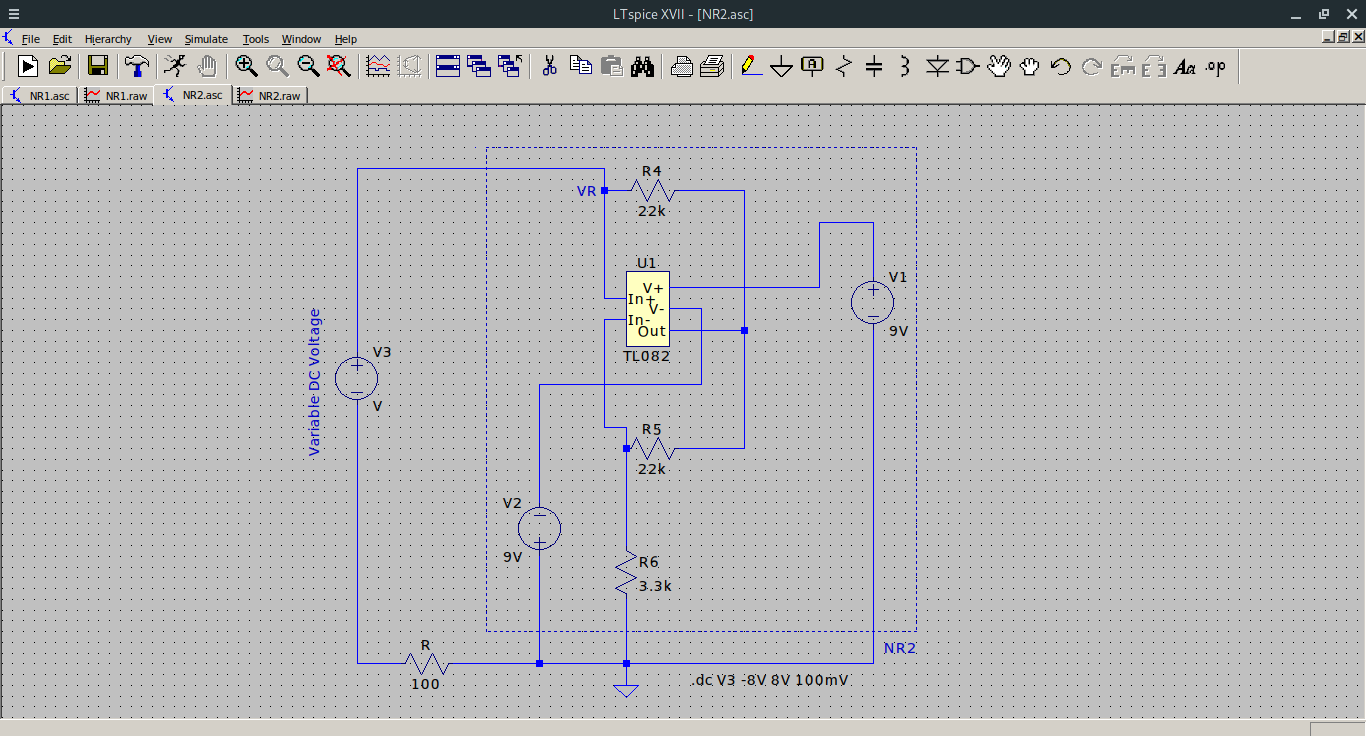
\includegraphics[width=\textwidth]{LTSpice/NR2_circuit.png}
	\caption{Fig 16. $N_{R_2}$ circuit}
\end{figure}
\begin{figure}[H]
	\centering
	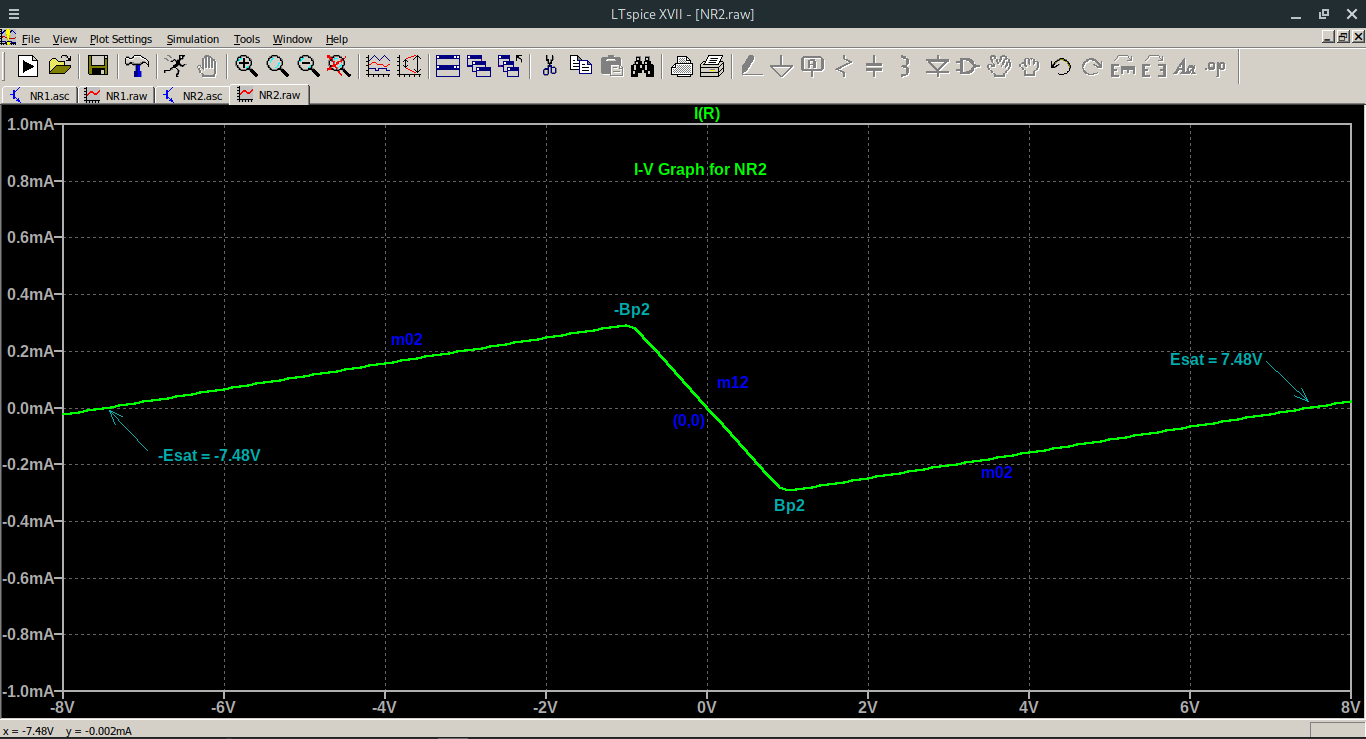
\includegraphics[width=\textwidth]{LTSpice/NR2_plot.png}
	\caption{Fig 17. I-V Characteristics of $N_{R_2}$}
\end{figure}
The values of slopes and breakpoints for $N_{R_2}$ are obtained from (\myref{eq:29}) as :
\begin{align*}
	E_{sat}&= \pm 7.48V \\
	m_{02}&=4.545\times 10^{-5}S = 0.04545 mS \\
	m_{12}&=-0.303\times 10^{-3}S = -0.303 mS \\
	B_{P2}&= \pm 0.976V
\end{align*}
%%
%subsection 5.3 - Non-Linear Resistance
\subsection{Non-Linear Resistance}
The Non-Linear negative resistance is implemented in LTSpice using two linear negative resistances in parallel. $V_3$ is a variable DC voltage source and R is a small resistance. 
\begin{figure}[H]
	\centering
	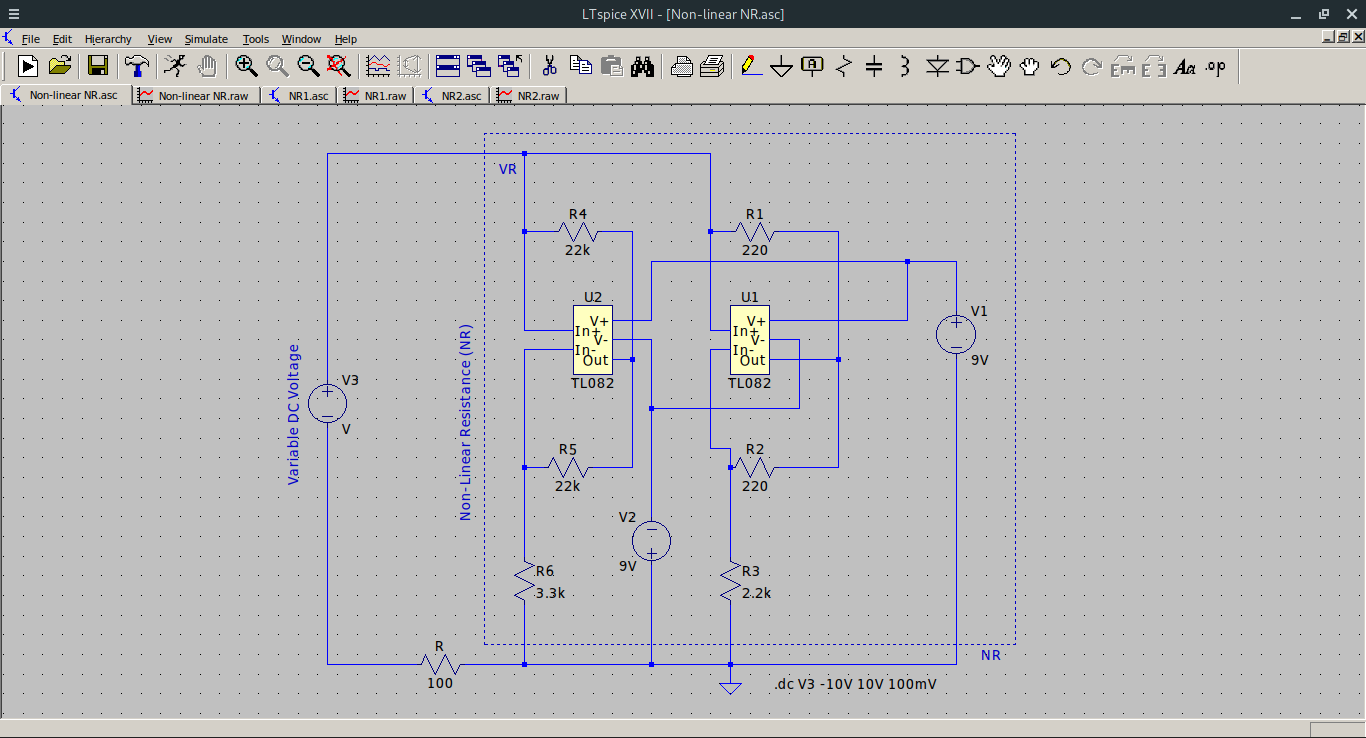
\includegraphics[width=\textwidth]{LTSpice/nonlinear NR_circuit.png}
	\caption{Fig 18. Non-Linear Negative Resistance $N_R$ circuit}
\end{figure}
To obtain the corresponding I-V graph, the circuit is run using DC Sweep mode from -10V to 10V with intervals of 100mV. The saturation voltage can be seen at $E_{sat}=\pm 7.48V$. 
\begin{figure}[H]
	\centering
	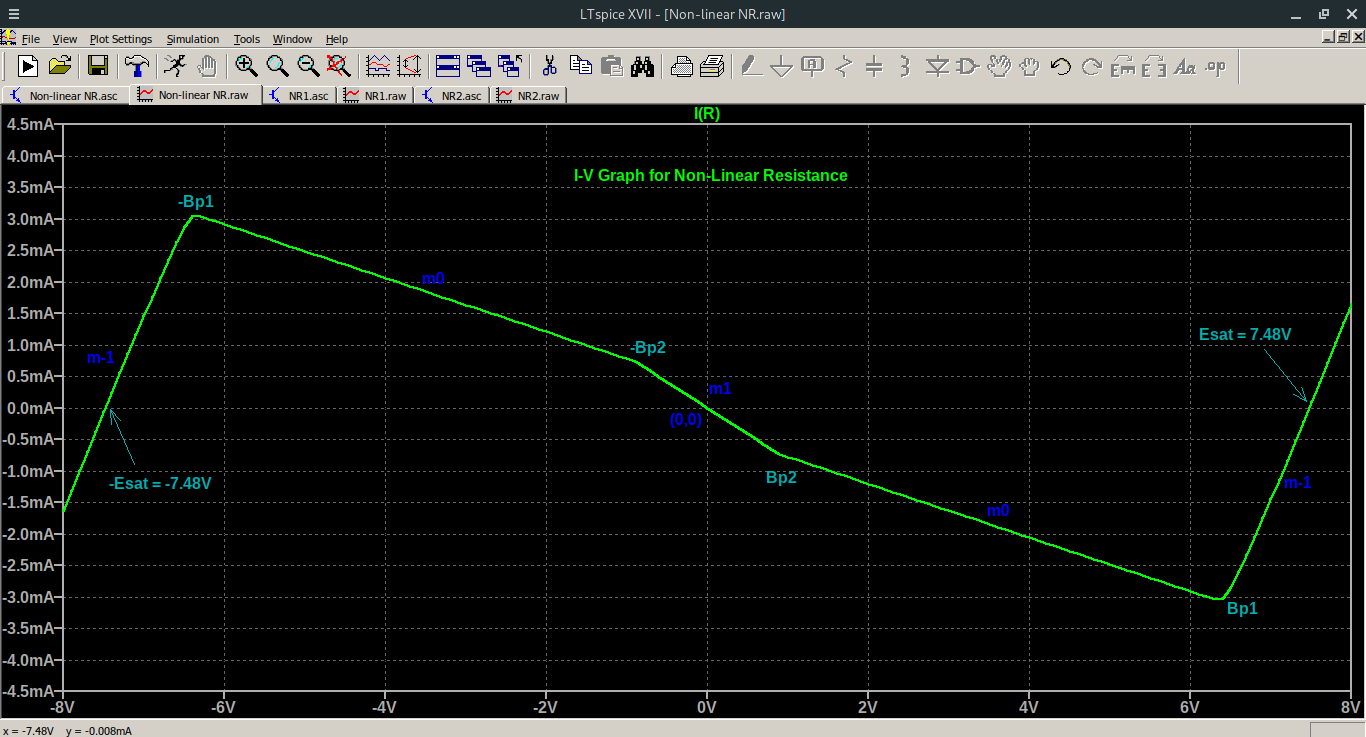
\includegraphics[width=\textwidth]{LTSpice/nonlinear NR_plot.png}
	\caption{Fig 19. I-V Characteristics Non-Linear Negative Resistance $N_R$}
\end{figure}
The slope of the graph can be calculated from (\myref{eq:30}) :
\begin{align*}
	m_0&=m_{11}+m_{02}=-0.4545+0.04545 =-0.4905 mS \\
	m_1&=m_{11}+m_{12}=-0.4545-0.303= -0.7575mS
\end{align*}
%%
%subsection 5.4 - Chua Circuit
\subsection{Chua Circuit}
Finally, Chua Circuit can be implemented in LTSpice using the non-linear resistance, a resistance ($R$) whose value we can vary from $2.2k\Omega$ to $1.2k\Omega$, two capacitances and one inductor. 
\begin{figure}[H]
	\centering
	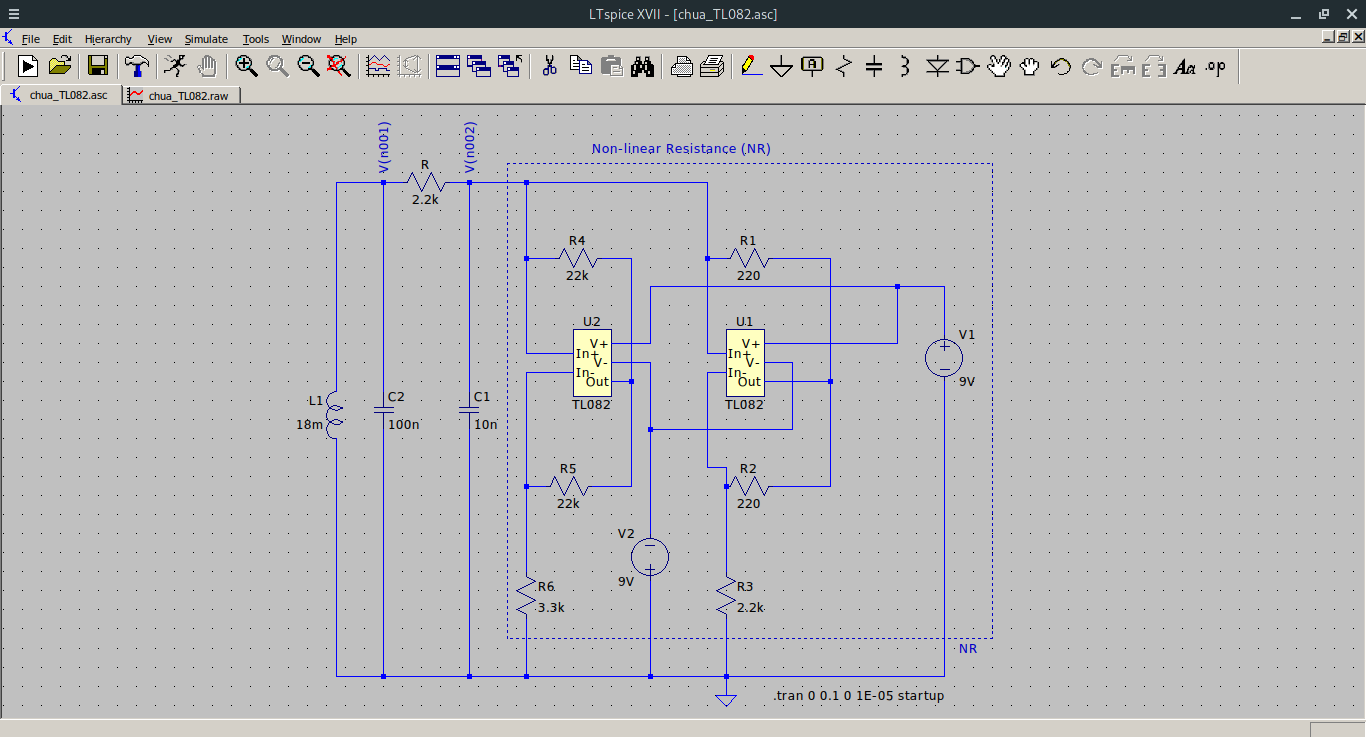
\includegraphics[width=\textwidth]{LTSpice/chua_circuit.png}
	\caption{Fig 20. Chua Circuit in LTSpice}
\end{figure}
The circuit is run in Transient mode. It runs for 0.1sec with maximum timestep being 1E-05sec. The data starts getting recorded at startup. \linebreak

To obtain the characteritics, we need to plot voltage across capacitance 1 ($v_{C1}$) in x-axis vs voltage across capacitance 2 ($v_{C2}$) in y-axis. In the LTSpice circuit :
\begin{align*}
	v_{C1} &\equiv \text{V(n002)} \\
	v_{C2} &\equiv \text{V(n001)}
\end{align*}
For different values of $R$ we stages of the bifurcation sequence, from period-0 to limit cycle. \linebreak
%R=2.2k
\subsubsection*{\romannum{1}. $R=2.2k\Omega$}
\begin{figure}[H] %2.2k
	\centering
	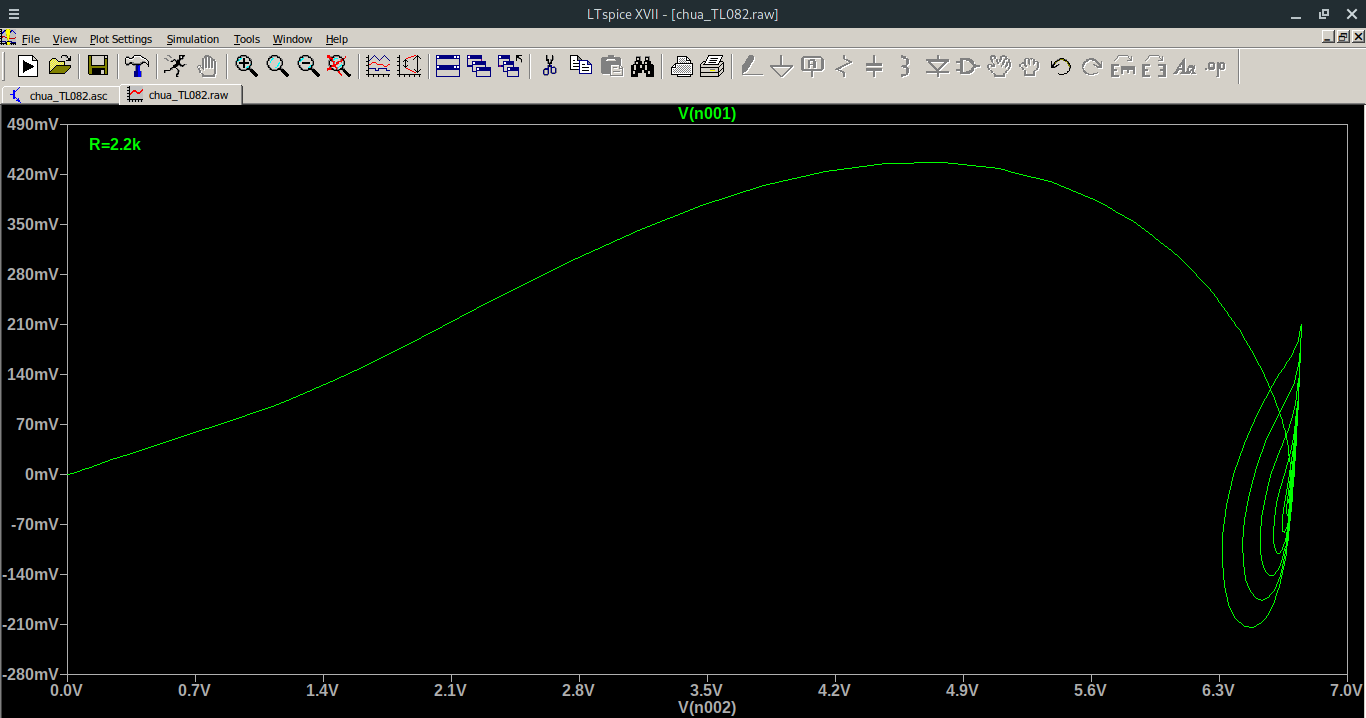
\includegraphics[width=\textwidth]{LTSpice/R=2.2k.png}
	\caption{Fig 21. $R=2.2k\Omega$}
\end{figure}
%R=2.1k
\subsubsection*{\romannum{2}. $R=2.1k\Omega$}
Period-0 of birfurcation sequence.
\begin{figure}[H] %2.1k
	\centering 
	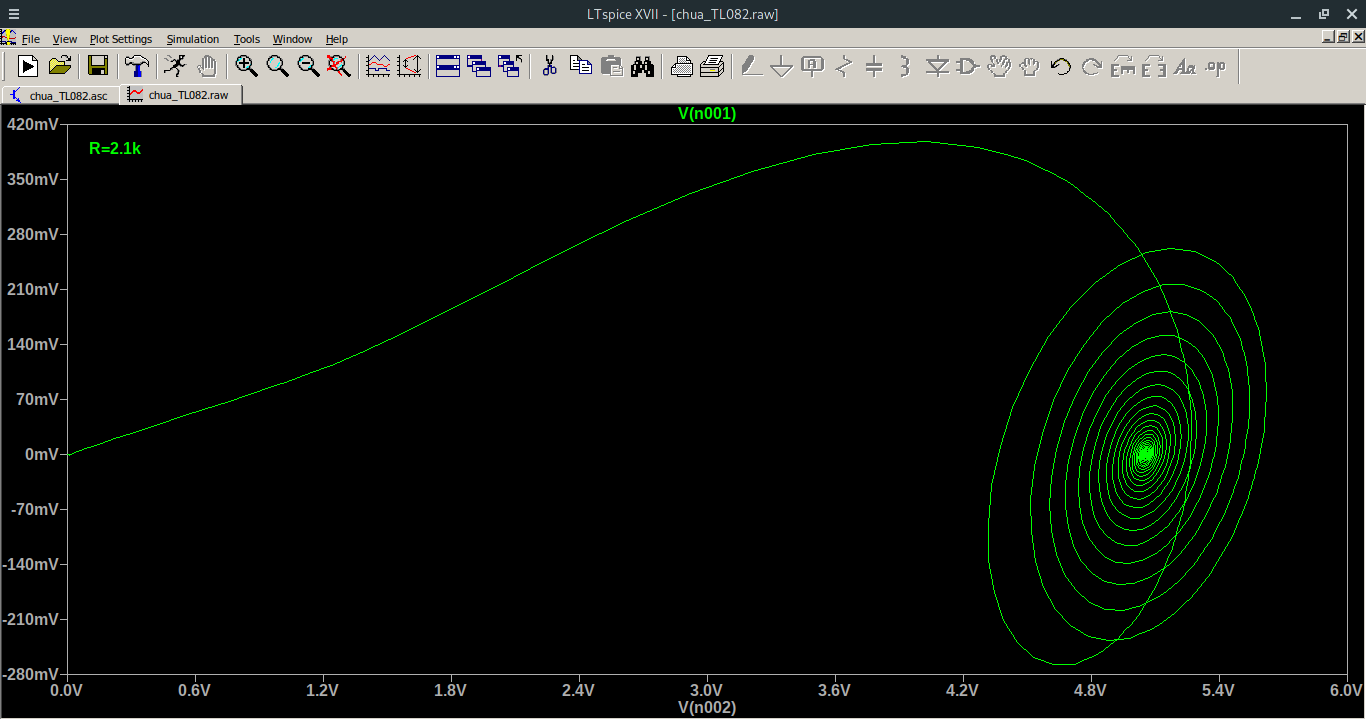
\includegraphics[width=\textwidth]{LTSpice/R=2.1k.png}
	\caption{Fig 22. $R=2.1k\Omega$ : Period-0}
\end{figure}
%R=1.96k
\subsubsection*{\romannum{3}. $R=1.96k\Omega$}
Period-1 of bifurcation sequence.
\begin{figure}[H] %1.96k
	\centering
	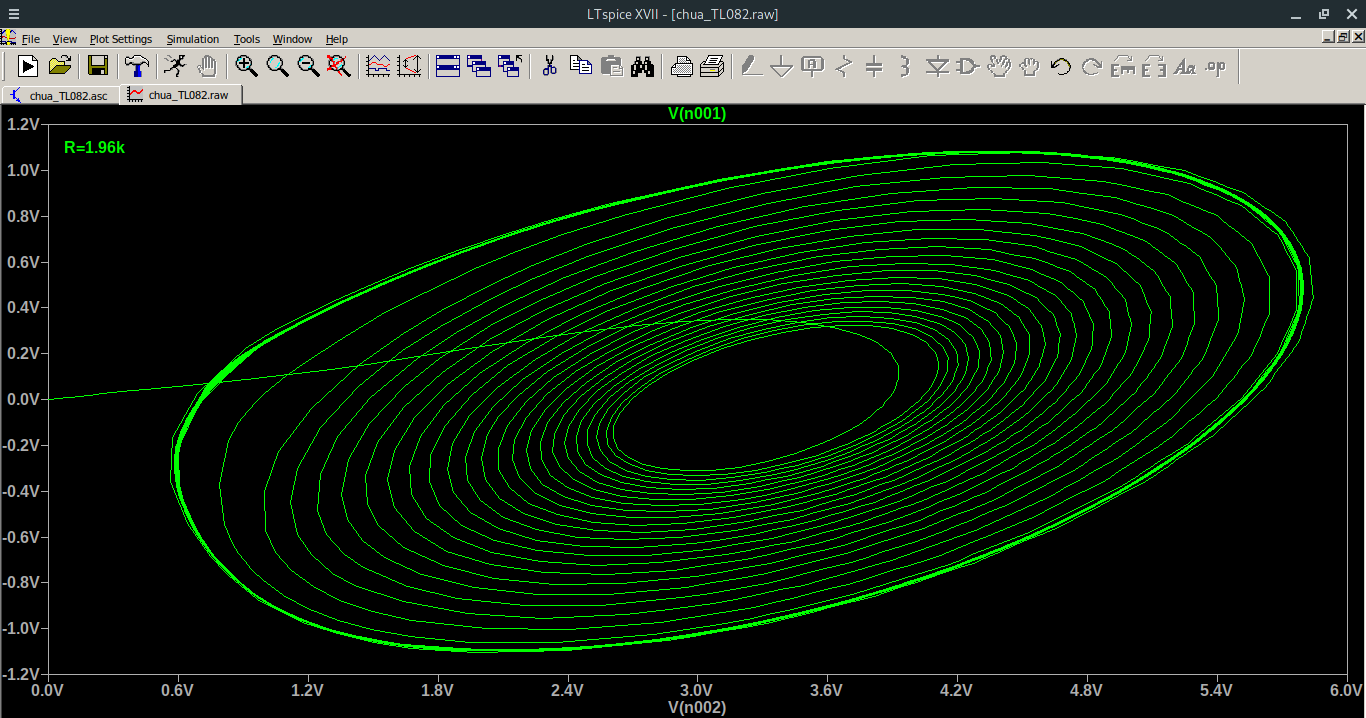
\includegraphics[width=\textwidth]{LTSpice/R=1.96k.png}
	\caption{Fig 23. $R=1.96k\Omega$ : Period-1}
\end{figure}
%R=1.94k
\subsubsection*{\romannum{4}. $R=1.94k\Omega$}
\begin{figure}[H] %1.94k
	\centering
	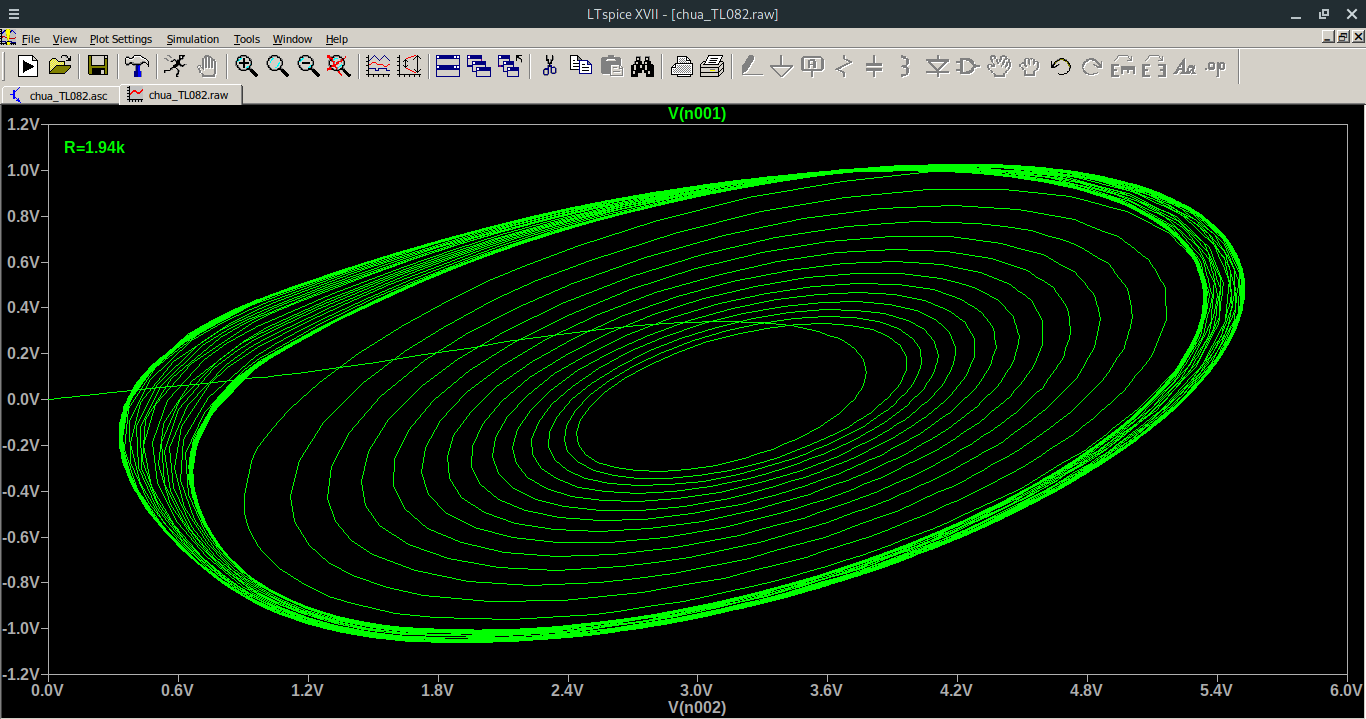
\includegraphics[width=\textwidth]{LTSpice/R=1.94k.png}
	\caption{Fig 24. $R=1.94k\Omega$}
\end{figure}
%R=1.935k
\subsubsection*{\romannum{5}. $R=1.935k\Omega$}
Period-2 of bifurcation sequence.
\begin{figure}[H] %1.935k
	\centering
	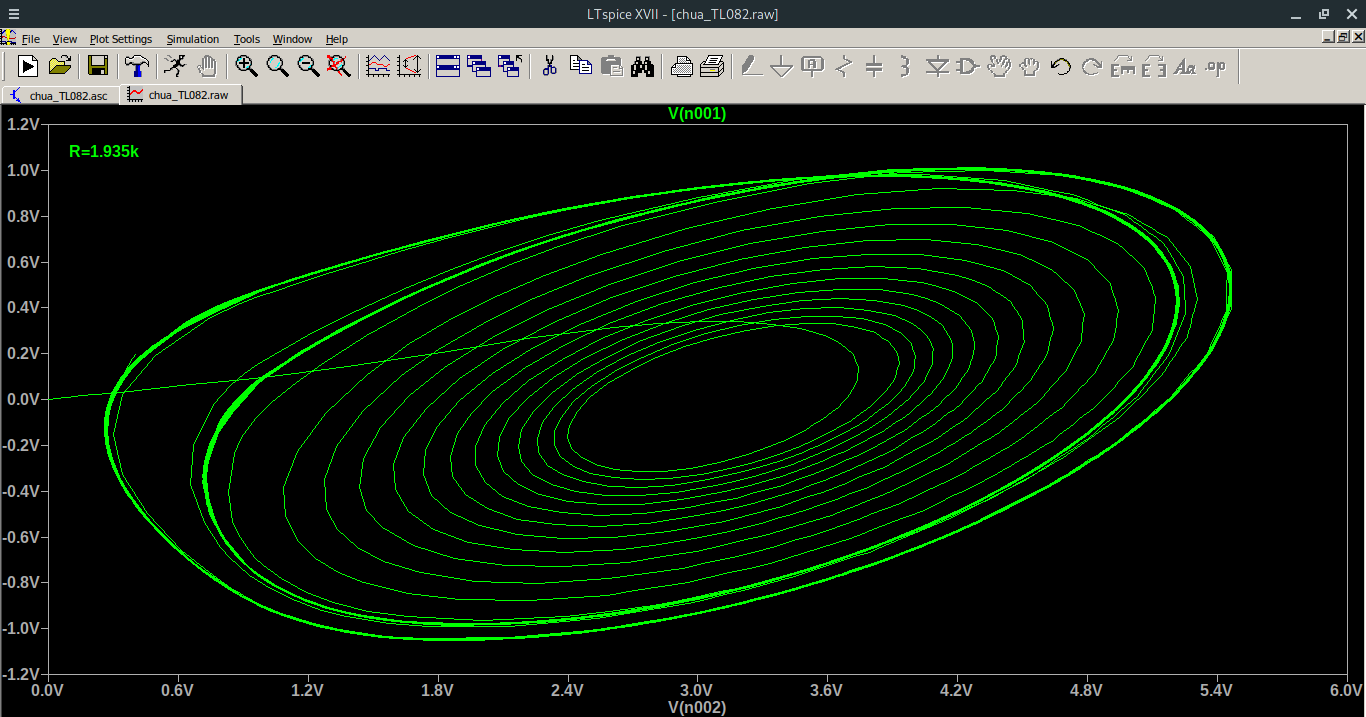
\includegraphics[width=\textwidth]{LTSpice/R=1.935k.png}
	\caption{Fig 25. $R=1.935k\Omega$ : Period-2}
\end{figure}
%R=1.927k
\subsubsection*{\romannum{6}. $R=1.927k\Omega$}
Period-4 of bifurcation sequence.
\begin{figure}[H] %1.927k
	\centering
	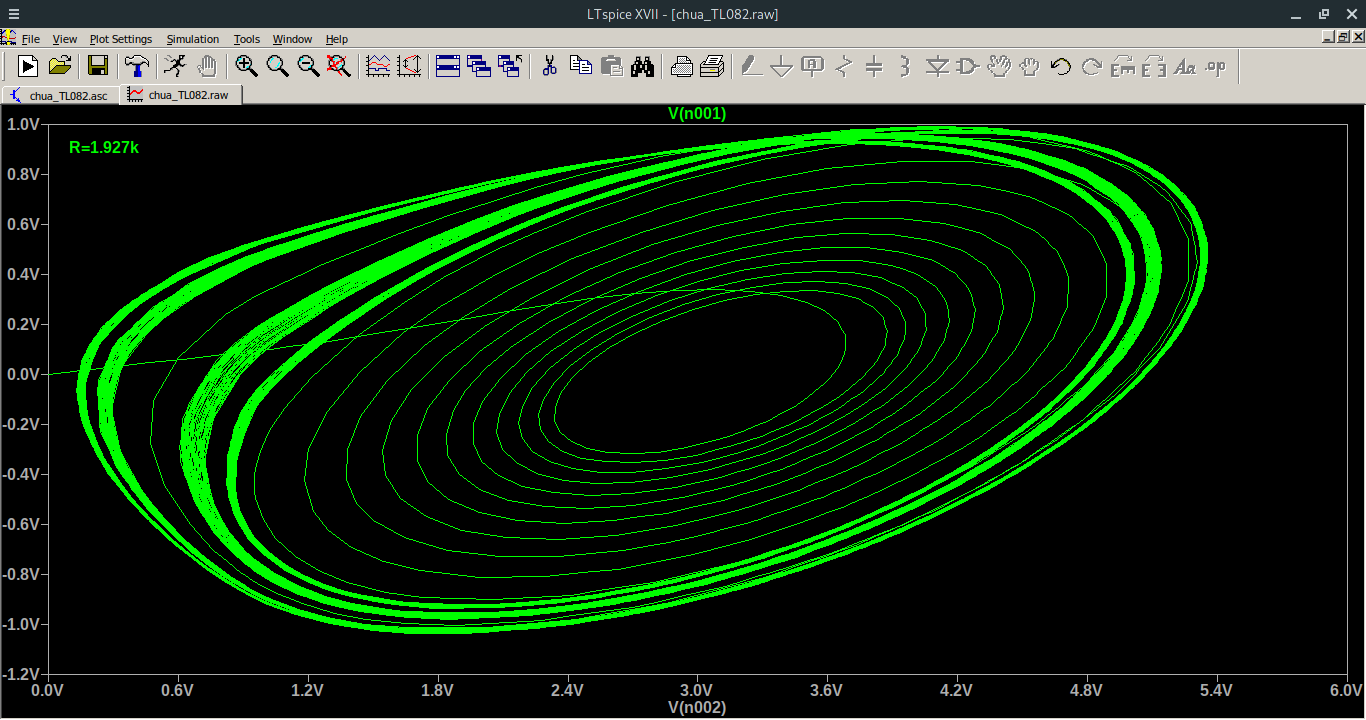
\includegraphics[width=\textwidth]{LTSpice/R=1.927k.png}
	\caption{Fig 26. $R=1.927k\Omega$ : Period-4}
\end{figure}
%R=1.91k
\subsubsection*{\romannum{7}. $R=1.91k\Omega$}
Period-3 window of bifurcation sequence.
\begin{figure}[H] %1.91k
	\centering
	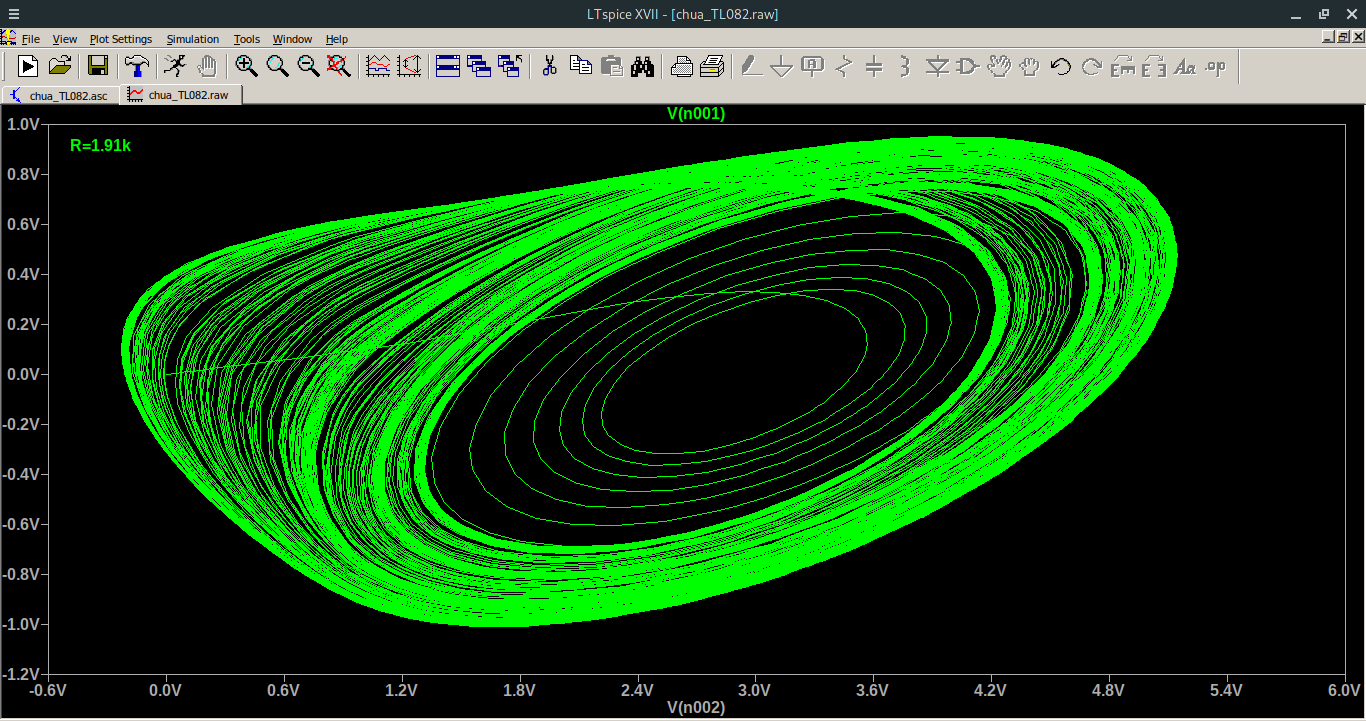
\includegraphics[width=\textwidth]{LTSpice/R=1.91k.png}
	\caption{Fig 27. $R=1.935k\Omega$ : Period-3 window}
\end{figure}
%R=1.90k
\subsubsection*{\romannum{8}. $R=1.90k\Omega$}
Rossler-type attractor of bifurcation sequence.
\begin{figure}[H] %1.90k
	\centering
	\includegraphics[width=\textwidth]{LTSpice/R=1.90k.png}
	\caption{Fig 28. $R=1.90k\Omega$ : Rossler-type attractor}
\end{figure}
%R=1.88k
\subsubsection*{\romannum{9}. $R=1.88k\Omega$}
Double Scroll attractor of bifurcation sequence.
\begin{figure}[H] %1.88k
	\centering
	\includegraphics[width=\textwidth]{LTSpice/R=1.88k.png}
	\caption{Fig 29. $R=1.88k\Omega$ : Double Scroll attractor}
\end{figure}
%R=1.80k
\subsubsection*{\romannum{10}. $R=1.80k\Omega$}
Double Scroll attractor, reducing in size.
\begin{figure}[H] %1.80k
	\centering
	\includegraphics[width=\textwidth]{LTSpice/R=1.80k.png}
	\caption{Fig 30. $R=1.80k\Omega$ : Double Scroll attractor}
\end{figure}
%R=1.70k
\subsubsection*{\romannum{11}. $R=1.70k\Omega$}
Double Scroll attractor, reducing in size.
\begin{figure}[H] %1.70k
	\centering
	\includegraphics[width=\textwidth]{LTSpice/R=1.70k.png}
	\caption{Fig 31. $R=1.70k\Omega$ : Double Scroll attractor}
\end{figure}
%R=1.60k
\subsubsection*{\romannum{12}. $R=1.60k\Omega$}
Double Scroll attractor, reducing in size.
\begin{figure}[H] %1.60k
	\centering
	\includegraphics[width=\textwidth]{LTSpice/R=1.60k.png}
	\caption{Fig 32. $R=1.60k\Omega$ : Double Scroll attractor}
\end{figure}
%R=1.50k
\subsubsection*{\romannum{13}. $R=1.50k\Omega$}
Double Scroll attractor, reducing in size.
\begin{figure}[H] %1.50k
	\centering
	\includegraphics[width=\textwidth]{LTSpice/R=1.50k.png}
	\caption{Fig 33. $R=1.50k\Omega$ : Double Scroll attractor}
\end{figure}
%R=1.48k
\subsubsection*{\romannum{14}. $R=1.48k\Omega$}
Limit cycle of the birfurcation sequence.
\begin{figure}[H] %1.48k
	\centering
	\includegraphics[width=\textwidth]{LTSpice/R=1.48k.png}
	\caption{Fig 34. $R=1.48k\Omega$ : Limit Cycle}
\end{figure}
Thus, we have obtained the entire bifurcation sequence of chua circuit starting from period-1 for $R=1.96k\Omega$ to limit cycle for $R=1.48k\Omega$. We can observe that unlike the simulation in Fig 5(n),(o),(p) the value of voltages does not shoot to arbitrarily large values. This is because we are dealing with a physically viable system which is eventually passive, as can be seen from the I-V Characteristics of Non-Linear resistor in Fig 19. 
%%%%%%%%%%%%%%%%%%%%%%%%%%%%%%%%%%%%%%%%%%%%%%%%%%%%
%section 6 - Inductorless Chua
\section{Inductorless Chua Circuit}
The inductor in Chua's Circuit produces oscillations in the circuit with the capacitance $C_2$. We can remove the inductor by using op-amps such that they mimic the behaviour of an inductor.
%%
%subsection 6.1 - Drawbacks of inductors
\subsection{Drawbacks of Inductors}
Even though inductors are very useful circuit elements, there are some disadvantages associated with them. 
\begin{enumerate}[i.]
	\item They are bigger and heavier than capacitors.
	\item As they store energy in form of magnetic fields, anytime a current passes through an inductor, a magnetic field is produced surrounding the wire.
	\item If we wish to have inductors store greater amount of energy, we need to have greater number of coils, which in turn increases the amount of magnetic field produced. This may interact with other circuit elements.
	\item If there are two or more inductors in the circuit, their magnetic fields may interact with each other. So, multiple inductors, if used, must be shielded from each other. 
	\item It is not easy to obtain inductors of any desired value. They are available in limited ranges.
\end{enumerate}
Thus, we would like to replace the inductor in the Chua Circuit with something that mimics the behaviour of an inductor.
%%
%subsection 6.2 - Op-Amps as Inductors
\subsection{Op-Amps as Inductors}
We can use op-amps to build synthetic inductors because op-amps can act as impedance converters, i.e., they can convert capacitances to inductors and vice versa. \linebreak

We can implement an inductor using op-amps as follows :
\begin{figure}[H]
	\centering
	\includegraphics[width=0.35\textwidth]{Images/fig35_opamp inductor.png}
	\caption{Fig 35. Inductor using Op-Amps}
\end{figure}
Here we can demand that $R_{10}$ is a variable resistor which allows us to define the value of the inductor we want to implement. \linebreak

The above circuit behaves as an inductor of value $L$ given as :
\begin{equation}
	L=\dfrac{R_7 R_9 R_{10} C}{R_8} \label{eq:31}
\end{equation}
%%
%subsection 6.3 - Implementing Inductorless Chua using LTSPice
\subsection{Implementing Inductorless Chua Circuit with LTSpice}
Inductorless Chua Circuit is implemented in LTSpice by replacing the $L$ in the original Chua Circuit with the circuit in Fig 35. \linebreak
All the op-amps used are TL082. \linebreak
The values of the components used for making the inductor :
\begin{align*}
	R_7&= 100\Omega \\
	R_8&=1.0k\Omega \\
	R_9&=1.0k\Omega \\
	R_{10}&=1.8k\Omega \\
	C&=100nF
\end{align*}
This gives us value of $L$ from (\myref{eq:31}) as :
\[ L=18mH \]
It is the same value of L as we used in our original Chua Circuit. 
\begin{figure}[H]
	\centering
	\includegraphics[width=\textwidth]{LTSpice/inductorless_chua.png}
	\caption{Fig 36. Inductorless Chua Circuit}
\end{figure}
The circuit is once again run in Transient mode. It runs for 0.1sec with maximum timestep being 1E-05sec. The data starts getting recorded at startup. \linebreak

To obtain the characteritics, we will plot voltage across capacitance 1 ($v_{C1}$) in x-axis vs voltage across capacitance 2 ($v_{C2}$) in y-axis. In the LTSpice circuit :
\begin{align*}
	v_{C1} &\equiv \text{V(n002)} \\
	v_{C2} &\equiv \text{V(n001)}
\end{align*}
We will vary values of $R$ from $2.2k\Omega$ to $1.48k\Omega$ and see if we obtain similar characteristics. \linebreak
If our implementation of the inductor is correct we should obtain similar graphs.
%R=2.2k
\subsubsection*{\romannum{1}. $R=2.2k\Omega$}
\begin{figure}[H] %2.2k
	\centering
	\includegraphics[width=\textwidth]{LTSpice/inductorless R=2.2k.png}
	\caption{Fig 37. $R=2.2k\Omega$}
\end{figure}
%R=2.1k
\subsubsection*{\romannum{2}. $R=2.1k\Omega$}
Period-0 of birfurcation sequence.
\begin{figure}[H] %2.1k
	\centering 
	\includegraphics[width=\textwidth]{LTSpice/inductorless R=2.1k.png}
	\caption{Fig 38. $R=2.1k\Omega$ : Period-0}
\end{figure}
%R=1.96k
\subsubsection*{\romannum{3}. $R=1.96k\Omega$}
Period-1 of bifurcation sequence.
\begin{figure}[H] %1.96k
	\centering
	\includegraphics[width=\textwidth]{LTSpice/inductorless R=1.96k.png}
	\caption{Fig 39. $R=1.96k\Omega$ : Period-1}
\end{figure}
%R=1.94k
\subsubsection*{\romannum{4}. $R=1.94k\Omega$}
Period-2 of bifurcation sequence.
\begin{figure}[H] %1.94k
	\centering
	\includegraphics[width=\textwidth]{LTSpice/inductorless R=1.94k.png}
	\caption{Fig 40. $R=1.94k\Omega$ : Period-2}
\end{figure}
%R=1.93k
\subsubsection*{\romannum{5}. $R=1.93k\Omega$}
Period-4 of bifurcation sequence.
\begin{figure}[H] %1.93k
	\centering
	\includegraphics[width=\textwidth]{LTSpice/inductorless R=1.93k.png}
	\caption{Fig 41. $R=1.93k\Omega$ : Period-4}
\end{figure}
%R=1.91k
\subsubsection*{\romannum{6}. $R=1.91k\Omega$}
Rossler-type attractor of bifurcation sequence.
\begin{figure}[H] %1.91k
	\centering
	\includegraphics[width=\textwidth]{LTSpice/inductorless R=1.91k.png}
	\caption{Fig 42. $R=1.91k\Omega$ : Rossler-type attractor}
\end{figure}
%R=1.89k
\subsubsection*{\romannum{7}. $R=1.89k\Omega$}
Double Scroll attractor of bifurcation sequence.
\begin{figure}[H] %1.89k
	\centering
	\includegraphics[width=\textwidth]{LTSpice/inductorless R=1.89k.png}
	\caption{Fig 43. $R=1.89k\Omega$ : Double Scroll attractor}
\end{figure}
%R=1.80k
\subsubsection*{\romannum{8}. $R=1.80k\Omega$}
Double Scroll attractor, reducing in size.
\begin{figure}[H] %1.80k
	\centering
	\includegraphics[width=\textwidth]{LTSpice/inductorless R=1.80k.png}
	\caption{Fig 44. $R=1.80k\Omega$ : Double Scroll attractor}
\end{figure}
%R=1.70k
\subsubsection*{\romannum{9}. $R=1.70k\Omega$}
Double Scroll attractor, reducing in size.
\begin{figure}[H] %1.70k
	\centering
	\includegraphics[width=\textwidth]{LTSpice/inductorless R=1.70k.png}
	\caption{Fig 45. $R=1.70k\Omega$ : Double Scroll attractor}
\end{figure}
%R=1.60k
\subsubsection*{\romannum{10}. $R=1.60k\Omega$}
Double Scroll attractor, reducing in size.
\begin{figure}[H] %1.60k
	\centering
	\includegraphics[width=\textwidth]{LTSpice/inductorless R=1.60k.png}
	\caption{Fig 46. $R=1.60k\Omega$ : Double Scroll attractor}
\end{figure}
%R=1.50k
\subsubsection*{\romannum{11}. $R=1.50k\Omega$}
Double Scroll attractor, reducing in size.
\begin{figure}[H] %1.50k
	\centering
	\includegraphics[width=\textwidth]{LTSpice/inductorless R=1.50k.png}
	\caption{Fig 47. $R=1.50k\Omega$ : Double Scroll attractor}
\end{figure}
%R=1.48k
\subsubsection*{\romannum{12}. $R=1.48k\Omega$}
Limit cycle of the birfurcation sequence.
\begin{figure}[H] %1.48k
	\centering
	\includegraphics[width=\textwidth]{LTSpice/inductorless R=1.48k.png}
	\caption{Fig 48. $R=1.48k\Omega$ : Limit Cycle}
\end{figure}

%%%%%%%%%%%%%%%%%%%%%%%%%%%%%%%%%%%%%%%%%%%%%%%%%%%%%%%%%%
%section 7 - Conclusion
\section{Summary and Conclusion}
Chua's circuit is one of the simplest method to observe chaos in a physical system. It consists of an inductor, two capacitors, a resistor and a non-linear resistor. 
\linebreak

The state equations of Chua Circuit is a set of three coupled differential equations given in (\myref{eq:1}), (\myref{eq:2}) and (\myref{eq:3}). The equations are solved using RK4 method for different values of $R$ and the results are plotted in Fig 5. It is observed that the results obtained are not physically viable as the non-linear characteristics used is not eventually passive. But nevertheless it still indicates that the Chua Circuit has the potential to show chaotic behaviour.\linebreak

To physically implement the Chua Circuit, first linear negative resistances are characterised theoretically using op-amps as Voltage Controlled Voltage Sources (VCVS). To obtain the non-linear resistance used in Chua's circuit, two negative resistances are joined in parallel. This gives us the required five-segment piecewise linear characteristics of the non-linear resistance. \linebreak

The circuits are physically implemented using LTSpice software. Each negative resistance $(N_{R_1}$ and $N_{R_2}$) is implemented and their I-V characteristics is obtained. Similarly non-linear resistance is obtained parallely joining $N_{R_1}$ and $N_{R_1}$. All I-V characteristics are obtained using a small current-sensing resistance $R=100\Omega$. The obtained I-V characteristics of all resistances ($N_{R_1}$, $N_{R_2}$ and $N_{R}$) matches the expected I-V characteristics. So our implementation is successful. $E_{sat}$ is measured to be $\pm 7.48V$. Breakpoints and slopes are calculated using the same. \linebreak

Finally Chua Circuit is also implemented using LTSpice and the value of $R$ is varied to obtain different graphs in the bifurcation sequence. Period-0 is obtained at $R=2.2k\Omega$, Period-1 at $R=1.96k\Omega$, Period-2 at $R=1.935k\Omega$, Period-4 at $R=1.927k\Omega$, Period-3 window at $R=1.91k\Omega$ and Rossler type attractor at $R=1.90k\Omega$, with sizes in decreasing order. Double scroll attractor first forms at $R=1.88k\Omega$ and as value of $R$ is decreased, the size of the double scroll decreases. At $R=1.48k\Omega$, the limit cycle is reached and the double scroll vanishes. \linebreak

Inductorless Chua Circuit is also implemented using LTSpice. The inductor was replaced by op-amps as shown in Fig 35. In the circuit, $R_{10}$ is kept as a variable resistor to control the value of inductance generated. While physically implementing the circuit, the circuit elements are so defined that $R_{10}=1.8k\Omega$ generates inductance $L=18mH$. The attractors of Inductorless Chua circuit are obtained at almost identical values of $R$ of the original circuit. Thus, we can say our implementation is successful.


%%%%%%%%%%%%%%%%%%%%%%% References %%%%%%%%%%%%%%%%%%%%%%
\nocite{*}
\bibliographystyle{ieeetr}
\bibliography{Ref}






\end{document}